\documentclass{beamer}

\usepackage[utf8]{inputenc}
\usepackage{graphicx}
\usepackage[backend=biber]{biblatex}
\bibliography{bibliography.bib}
\graphicspath{ {./images/} }
\usetheme{Warsaw}
%\usecolortheme{beaver}
%Information to be included in the title page:
\title[Trayectorias ortogonales monocromáticas ajenas] %optional
{Trayectorias ortogonales monocromáticas ajenas}
\subtitle{}
\author[Rodrigo Chávez] % (optional, for multiple authors)
{C.~J.~Rodrigo~Guadalupe\inst{1}}
\institute[VFU] % (optional)
{
  \inst{1}%
  Instituto de Matemáticas\\
  Universidad Nacional Autónoma de México

}

\date[VNL 2020] % (optional)
{XXXV Coloquio Victor Neumann Lara, Marzo 2020}



\begin{document}

\frame{\titlepage}


\begin{frame}
Para un punto $x$ en el plano una línea en forma de $L$ consistente de dos rayos, uno vertical y otro horizontal emanentes de $x$ es llamado L-línea con $esquina \, en \, x$
\end{frame}
\begin{frame}
\begin{figure}[h]
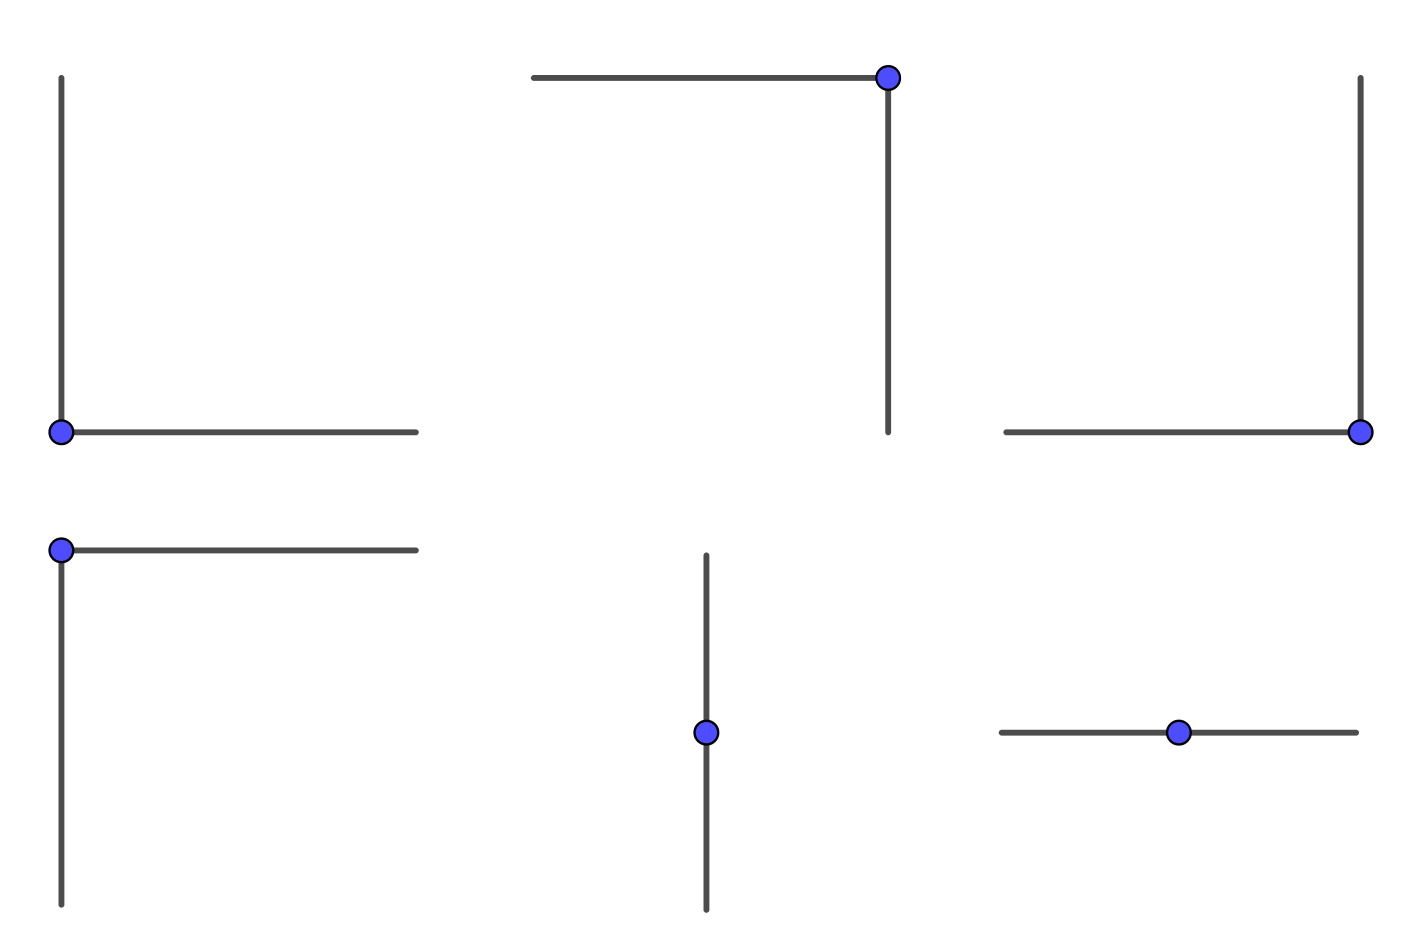
\includegraphics[width=\textwidth]{L-lineas}
\end{figure}
\end{frame}
\begin{frame}
\begin{figure}[h]
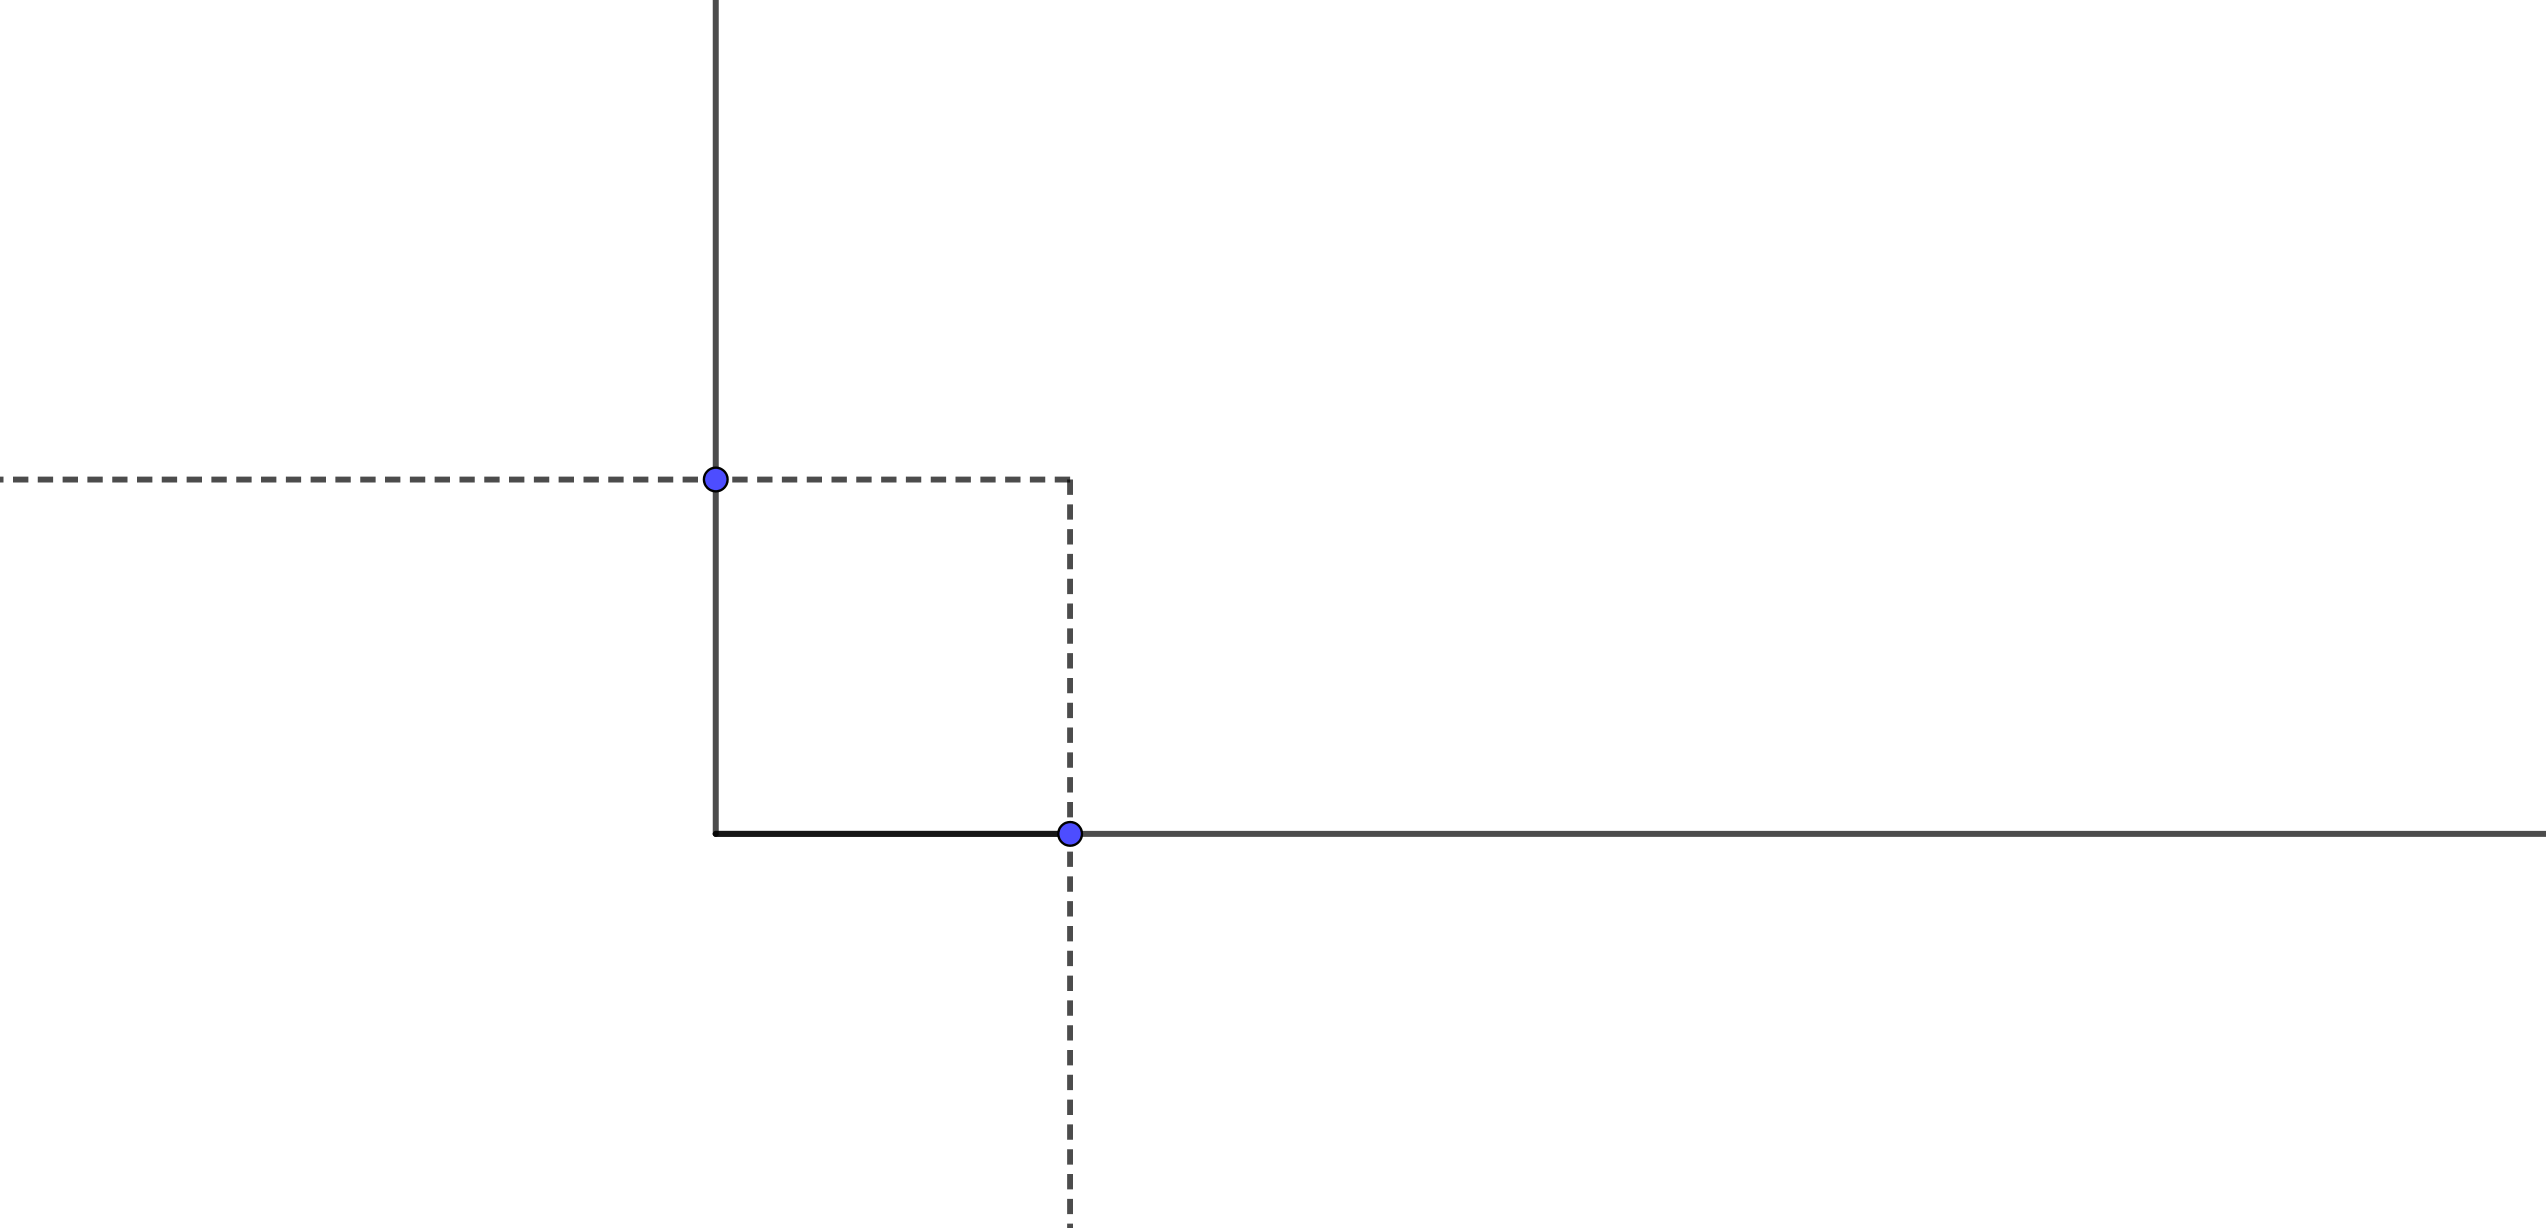
\includegraphics[width=\textwidth]{Diferencia-de-lineas-y-L-lineas}
\end{figure}
\end{frame}
\begin{frame}
\begin{figure}[h]
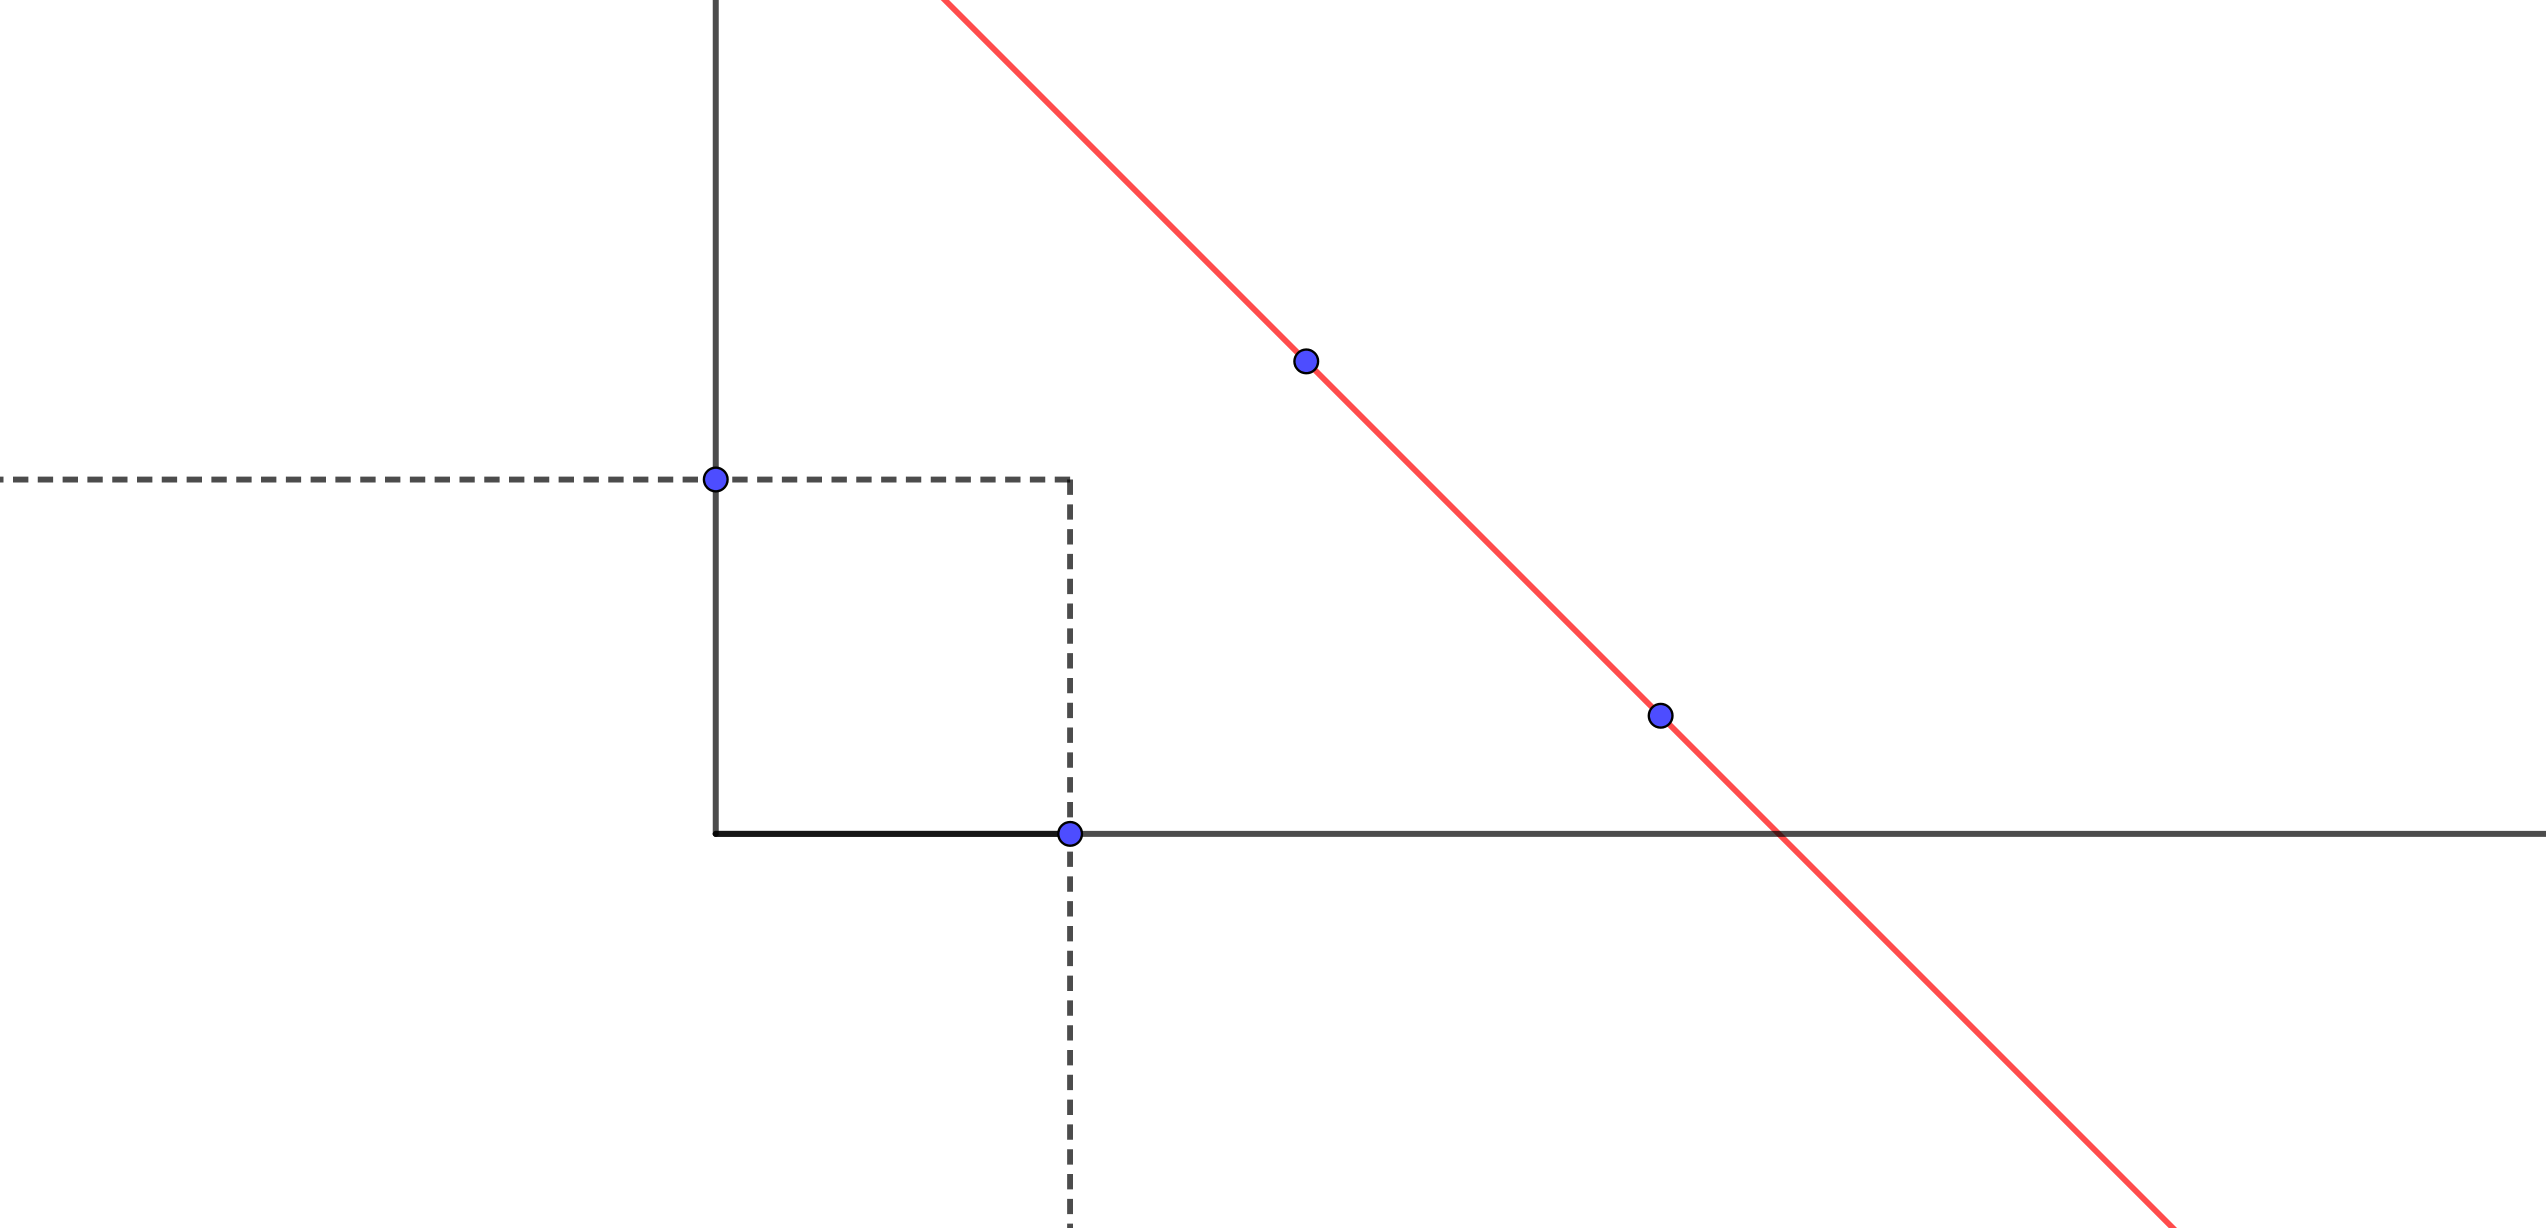
\includegraphics[width=\textwidth]{Diferencia-de-lineas-y-L-lineas-2}
\end{figure}
\end{frame}
\begin{frame}
\begin{figure}[h]
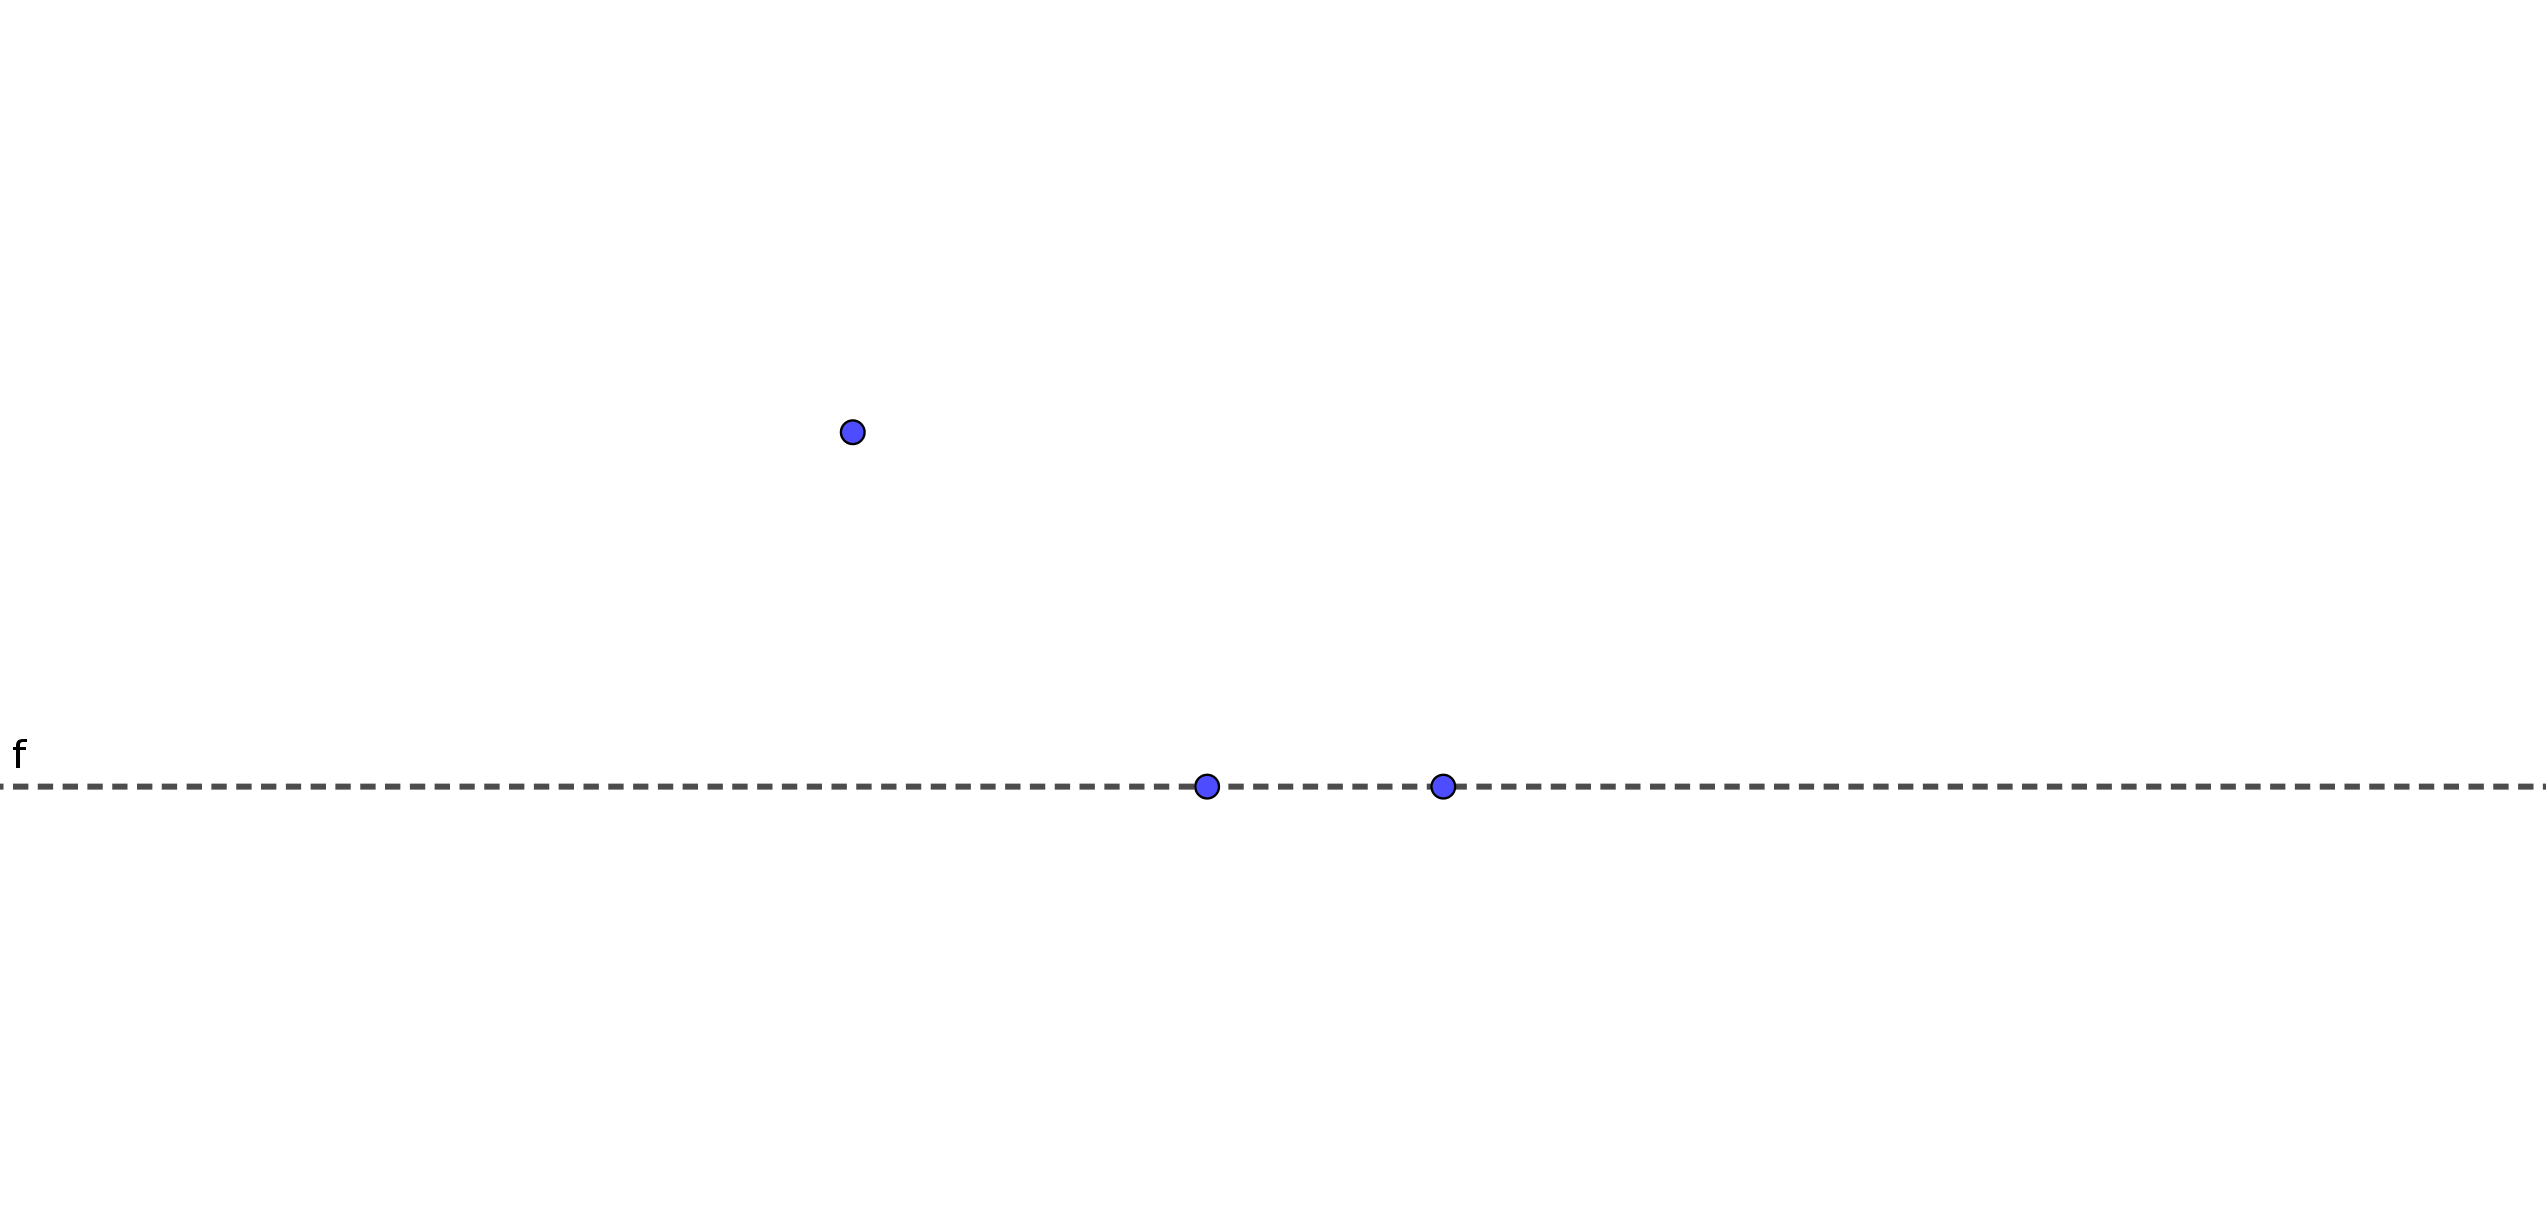
\includegraphics[width=\textwidth]{Posicion-general}
\end{figure}
\end{frame}
\begin{frame}
\begin{figure}[h]
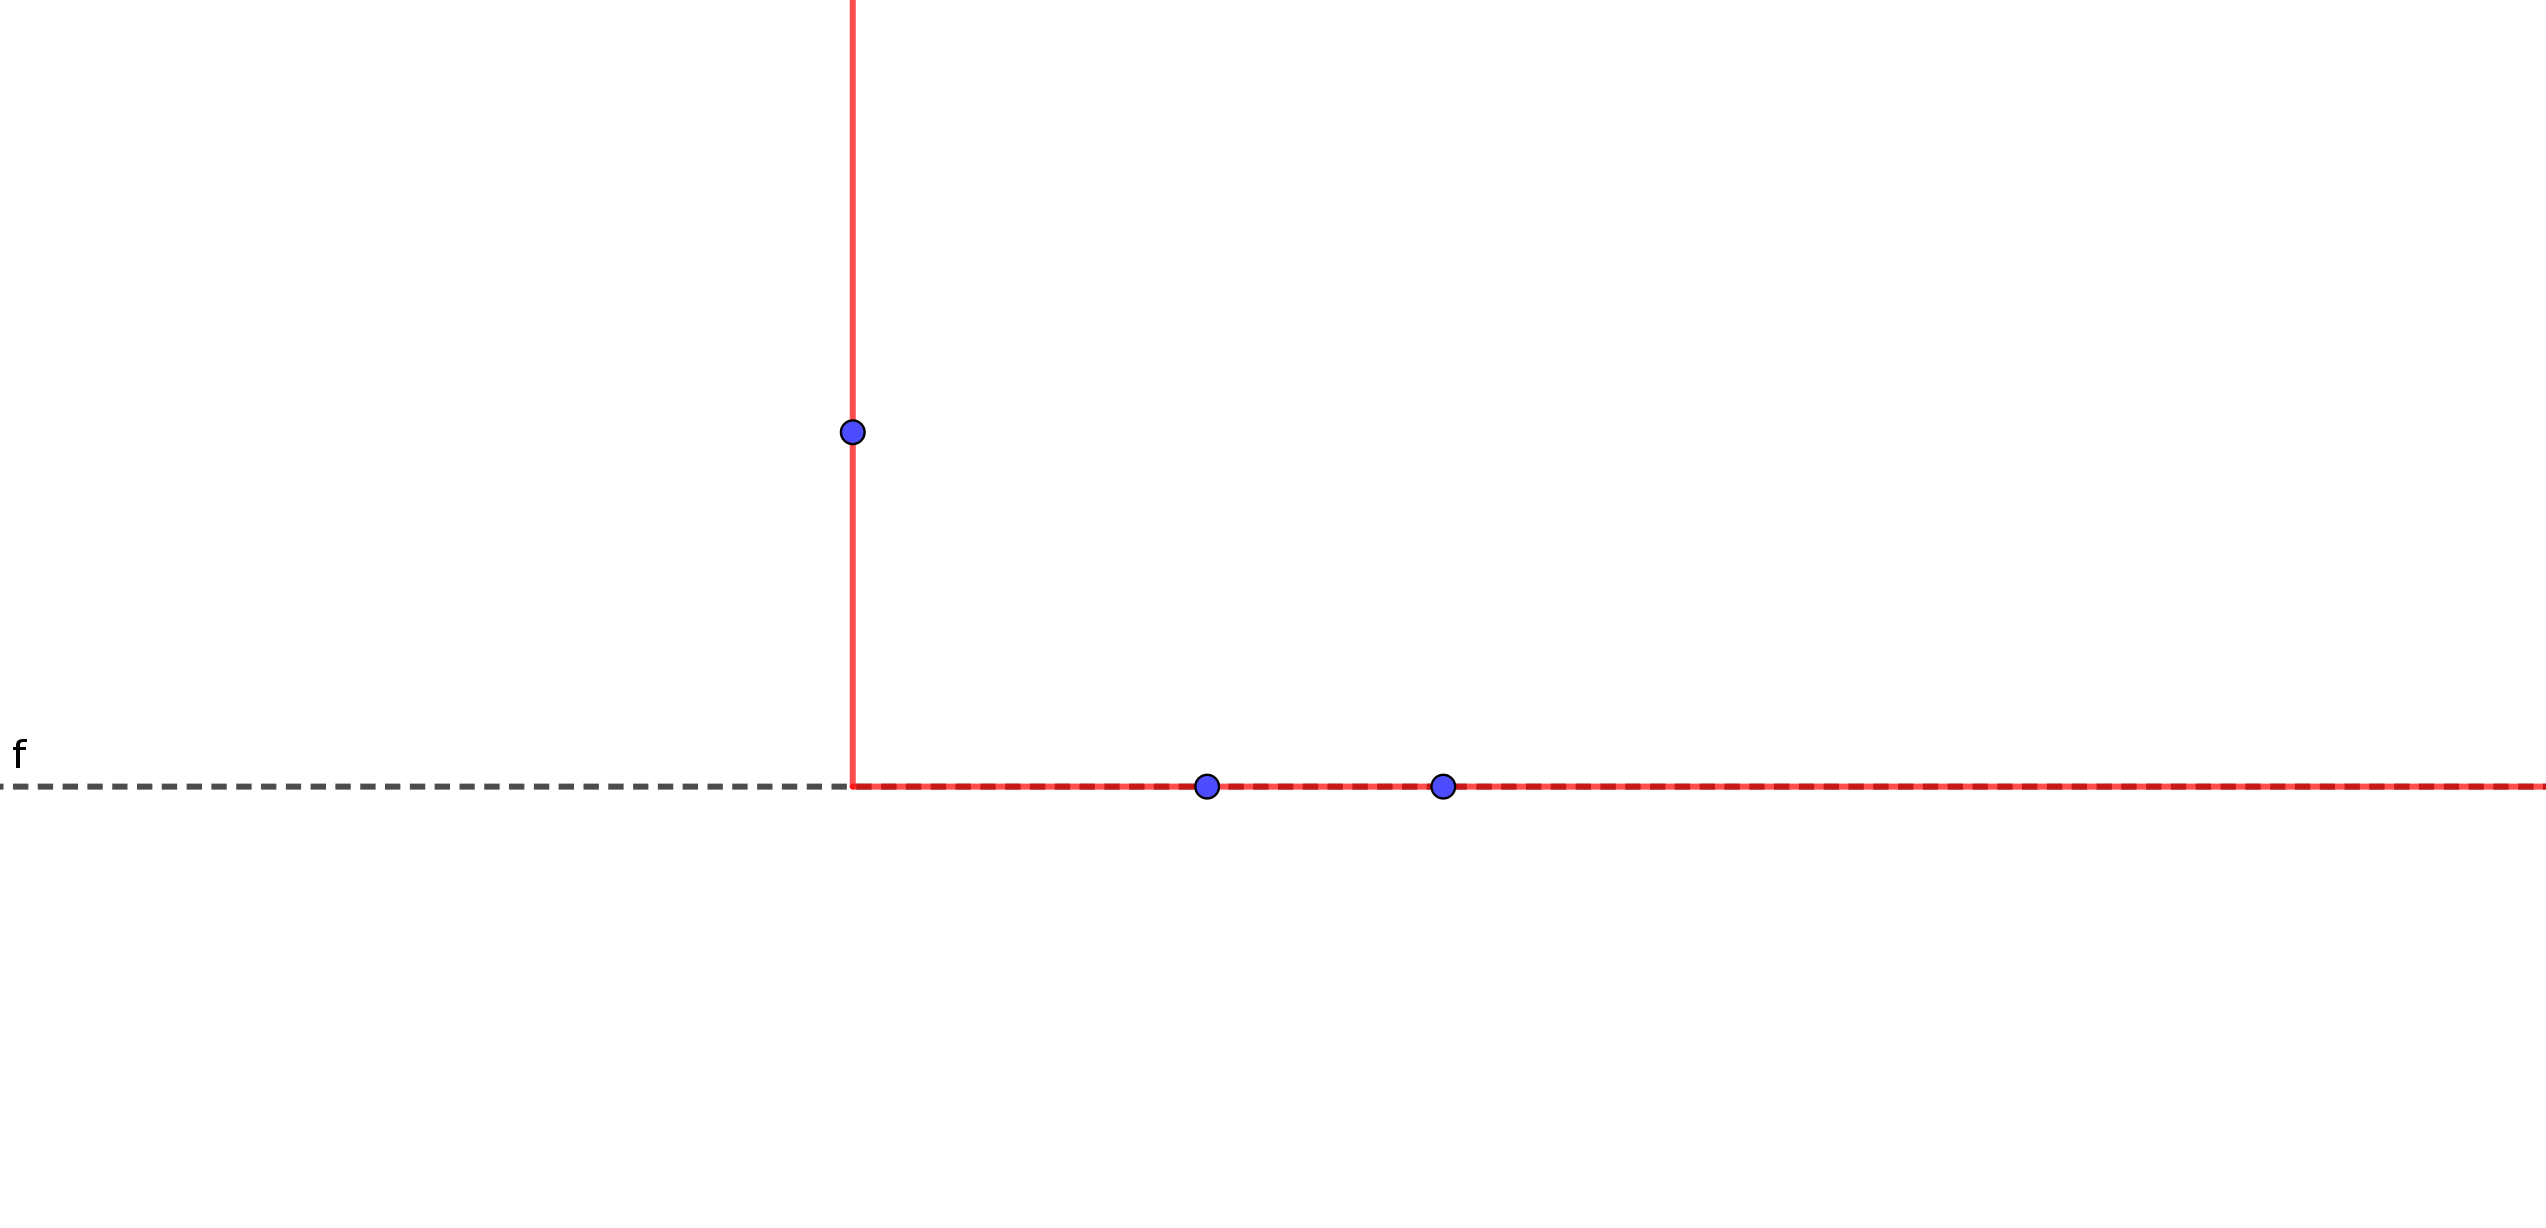
\includegraphics[width=\textwidth]{Posicion-general-2}
\end{figure}
\end{frame}
\begin{frame}
\begin{figure}[h]
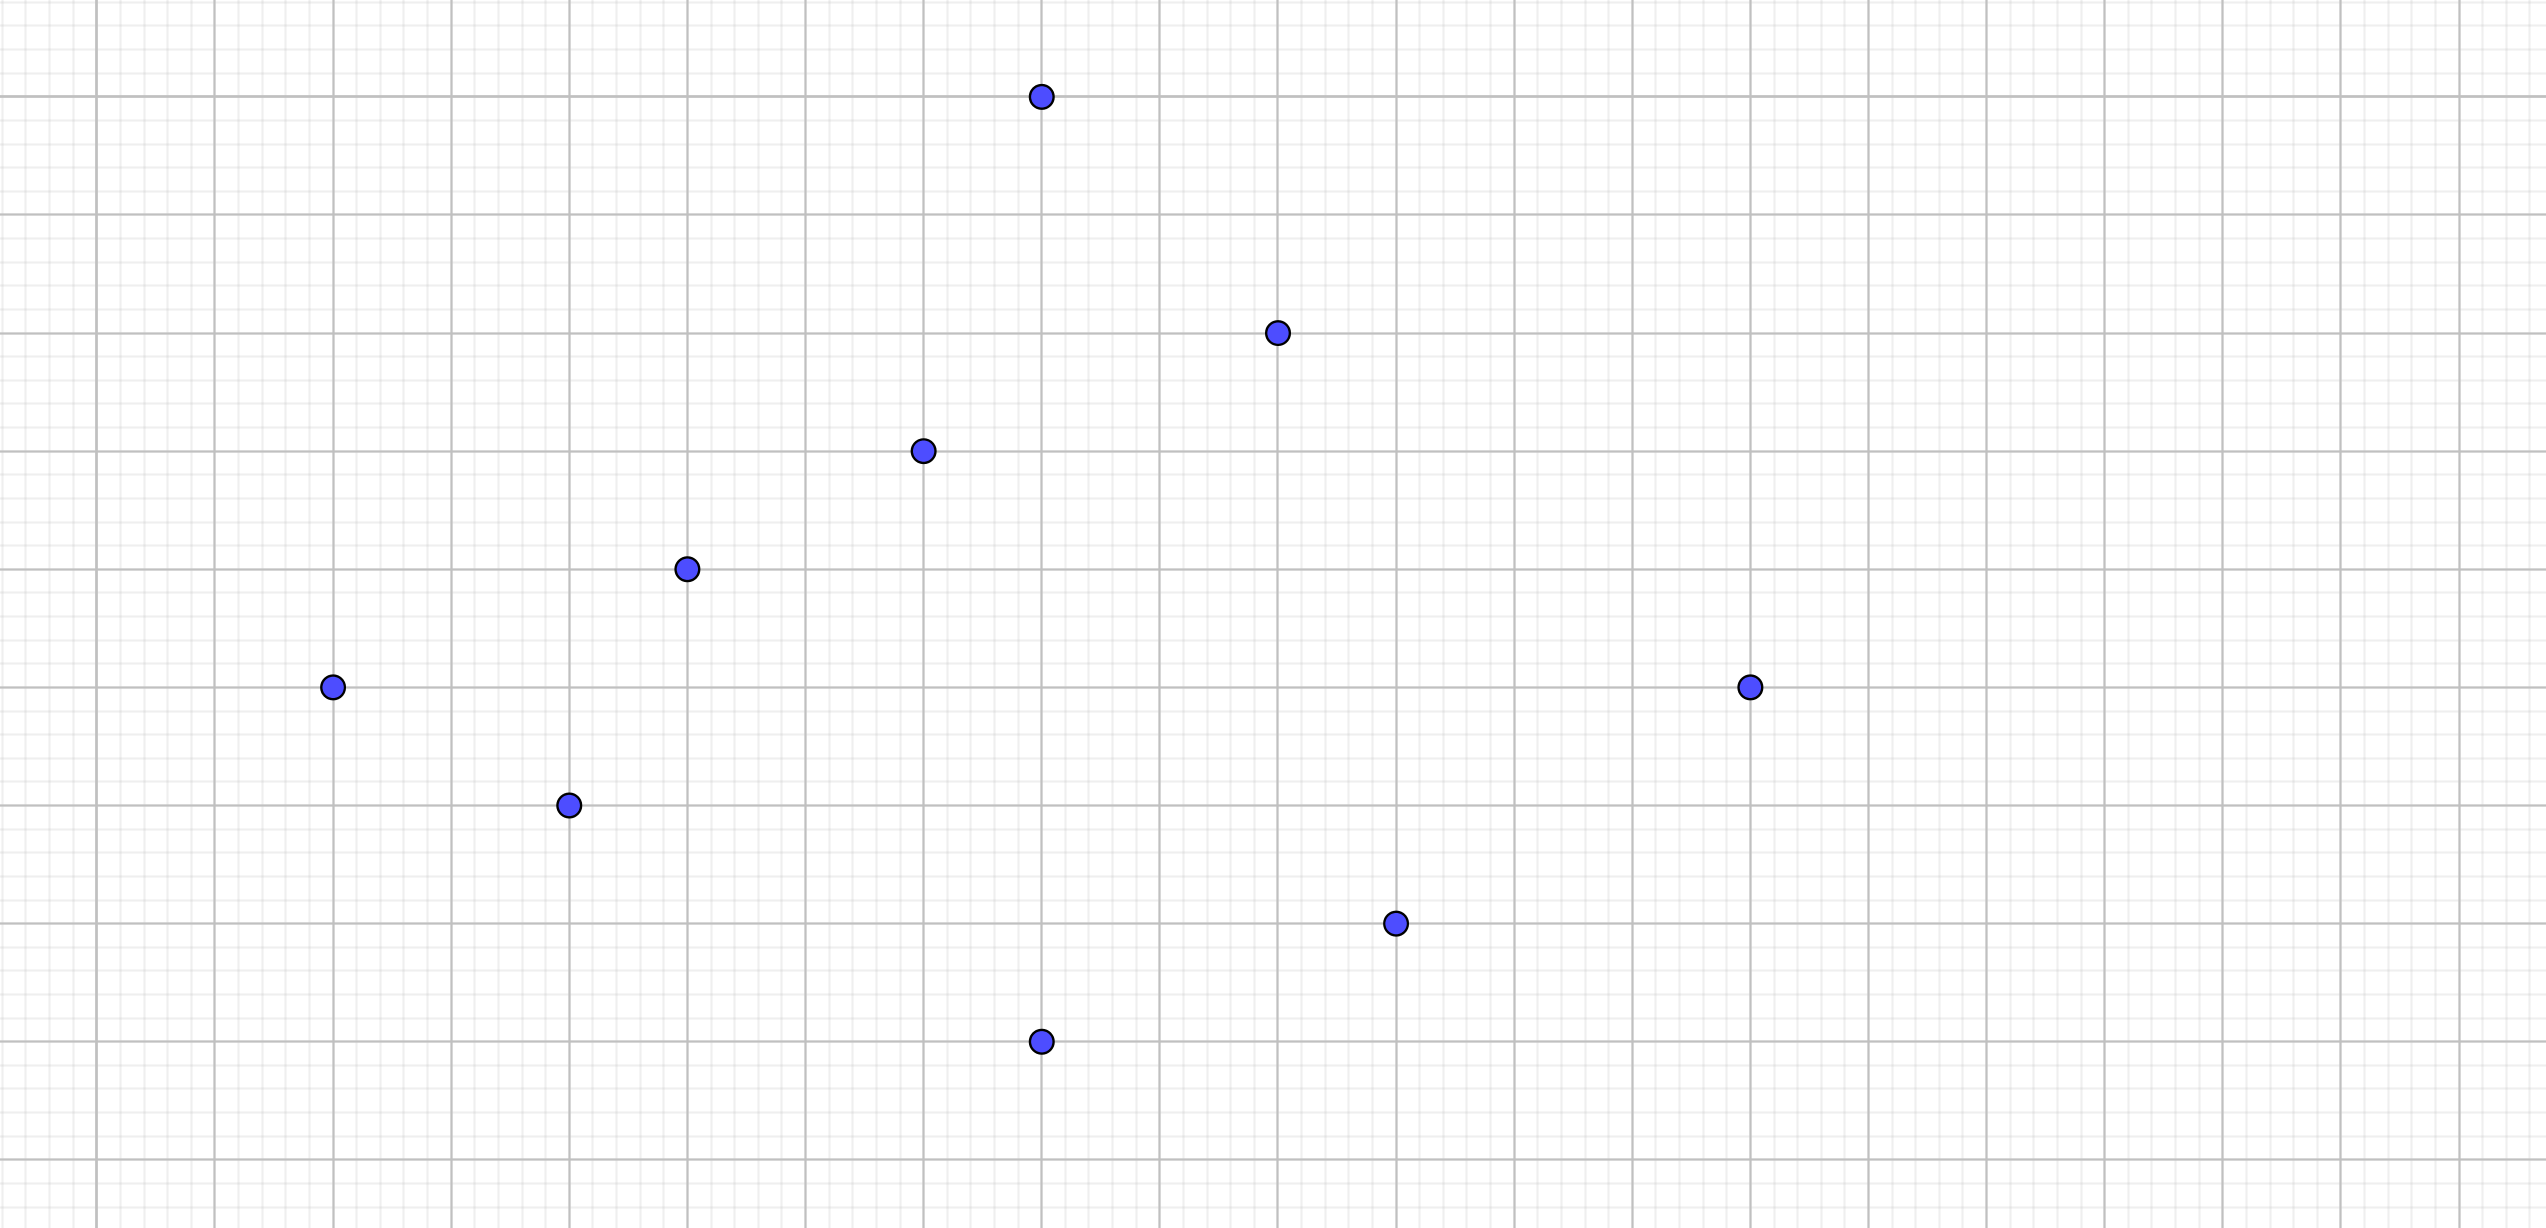
\includegraphics[width=\textwidth]{Prueba-misma-vertical}
\end{figure}
\end{frame}
\begin{frame}
\begin{figure}[h]
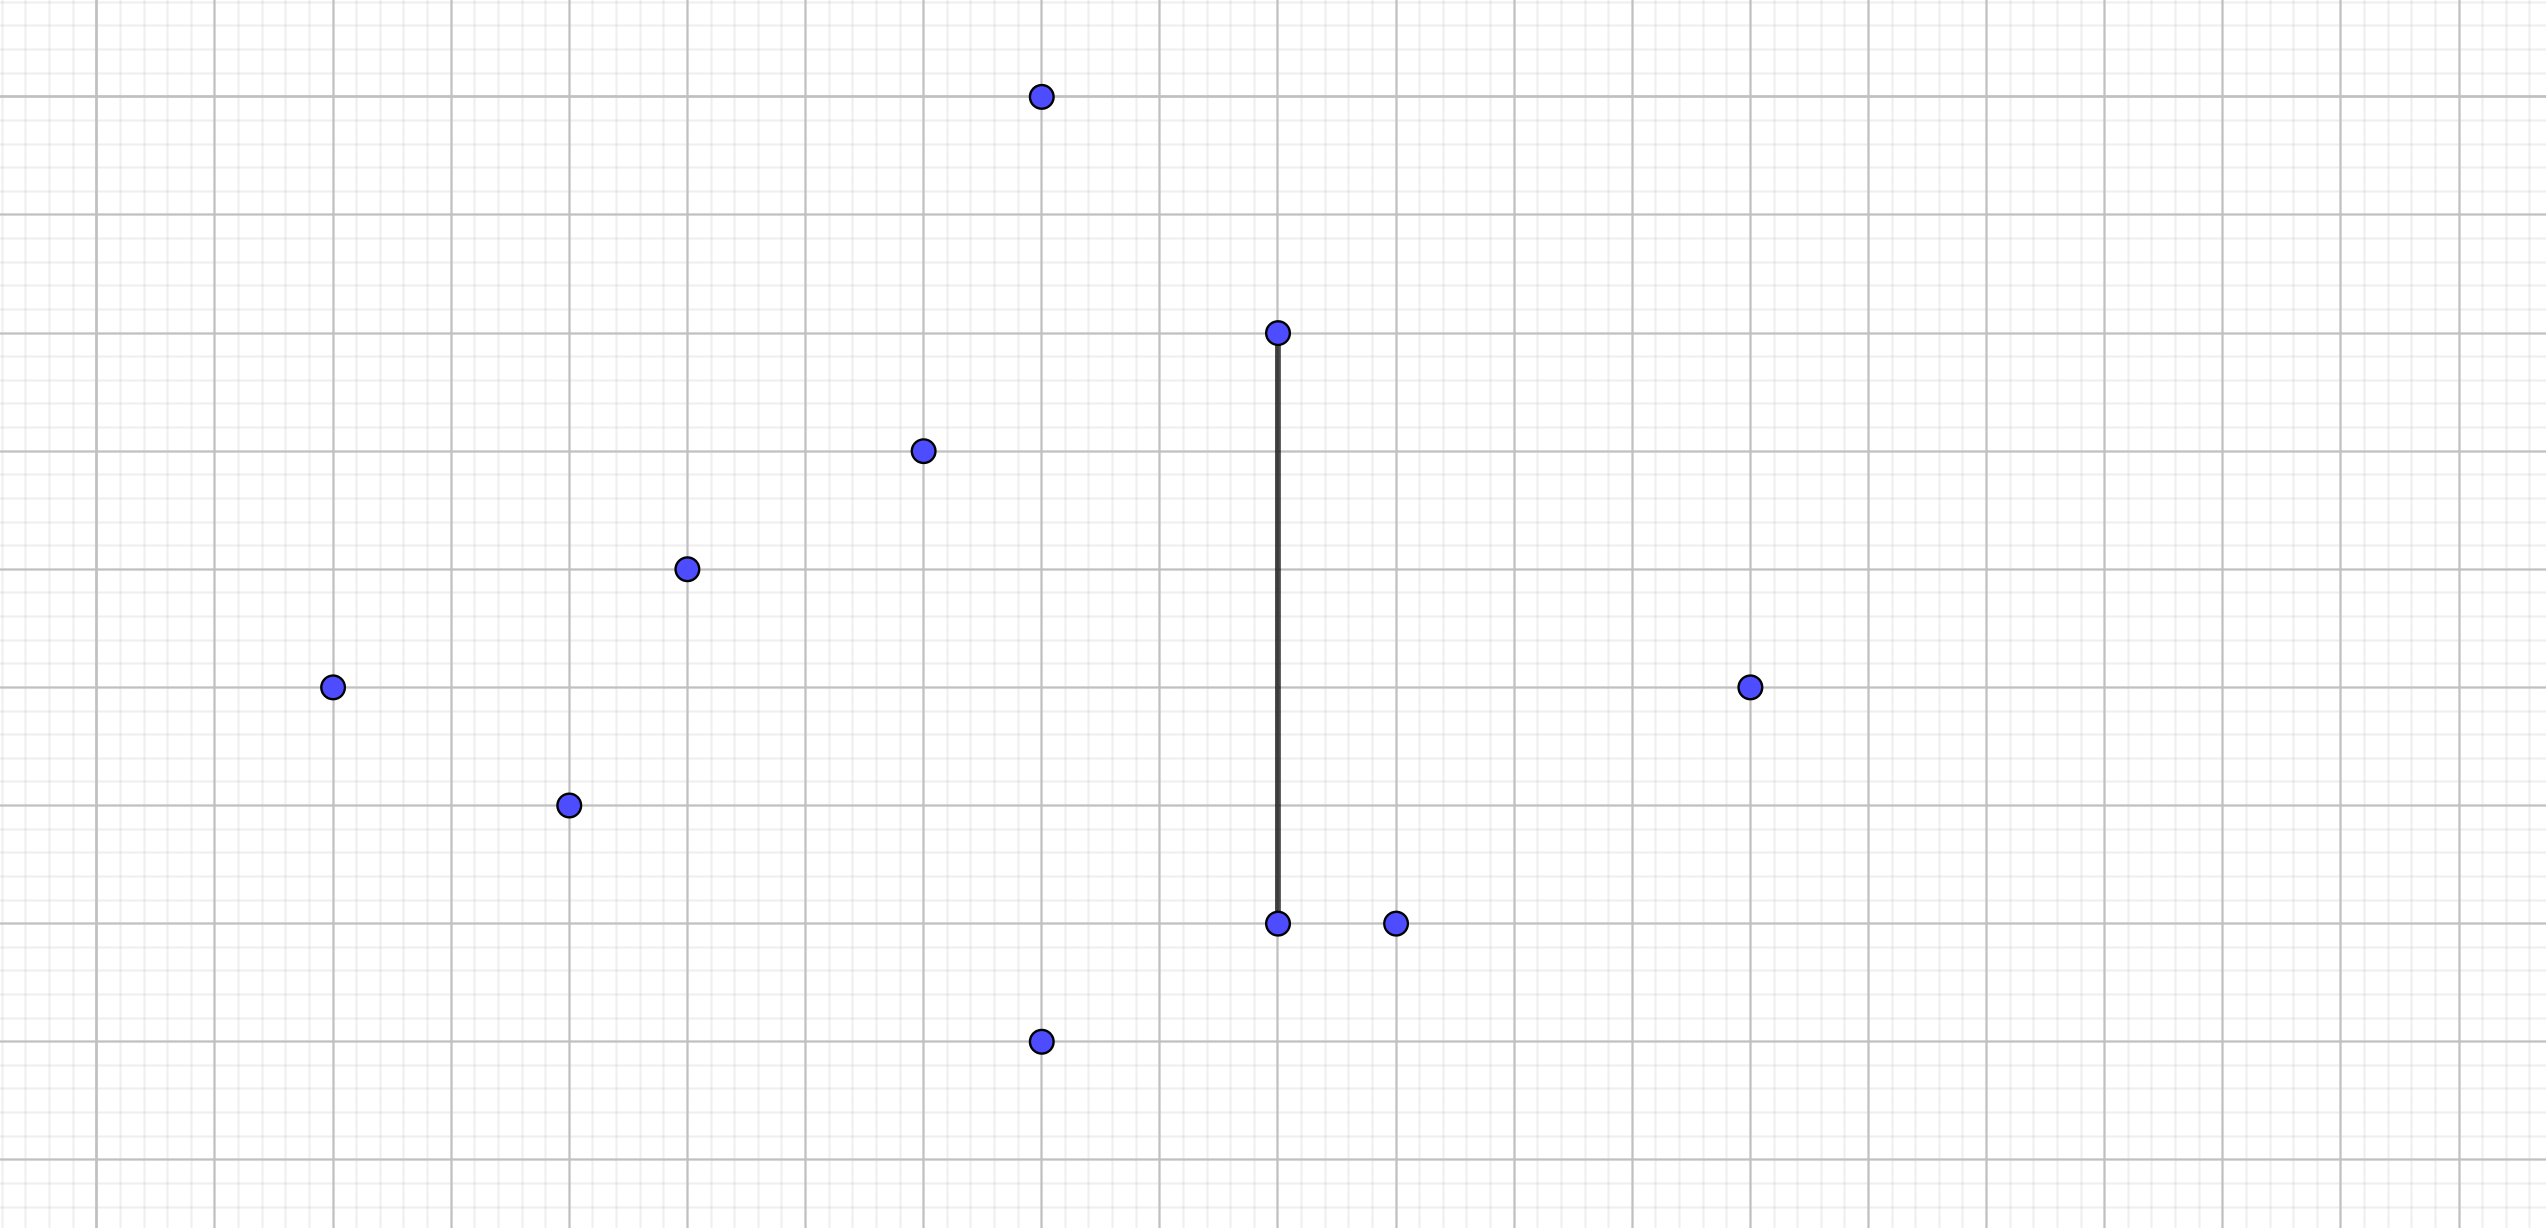
\includegraphics[width=\textwidth]{Prueba-misma-vertical-2}
\end{figure}
\end{frame}
\begin{frame}
\begin{figure}[h]
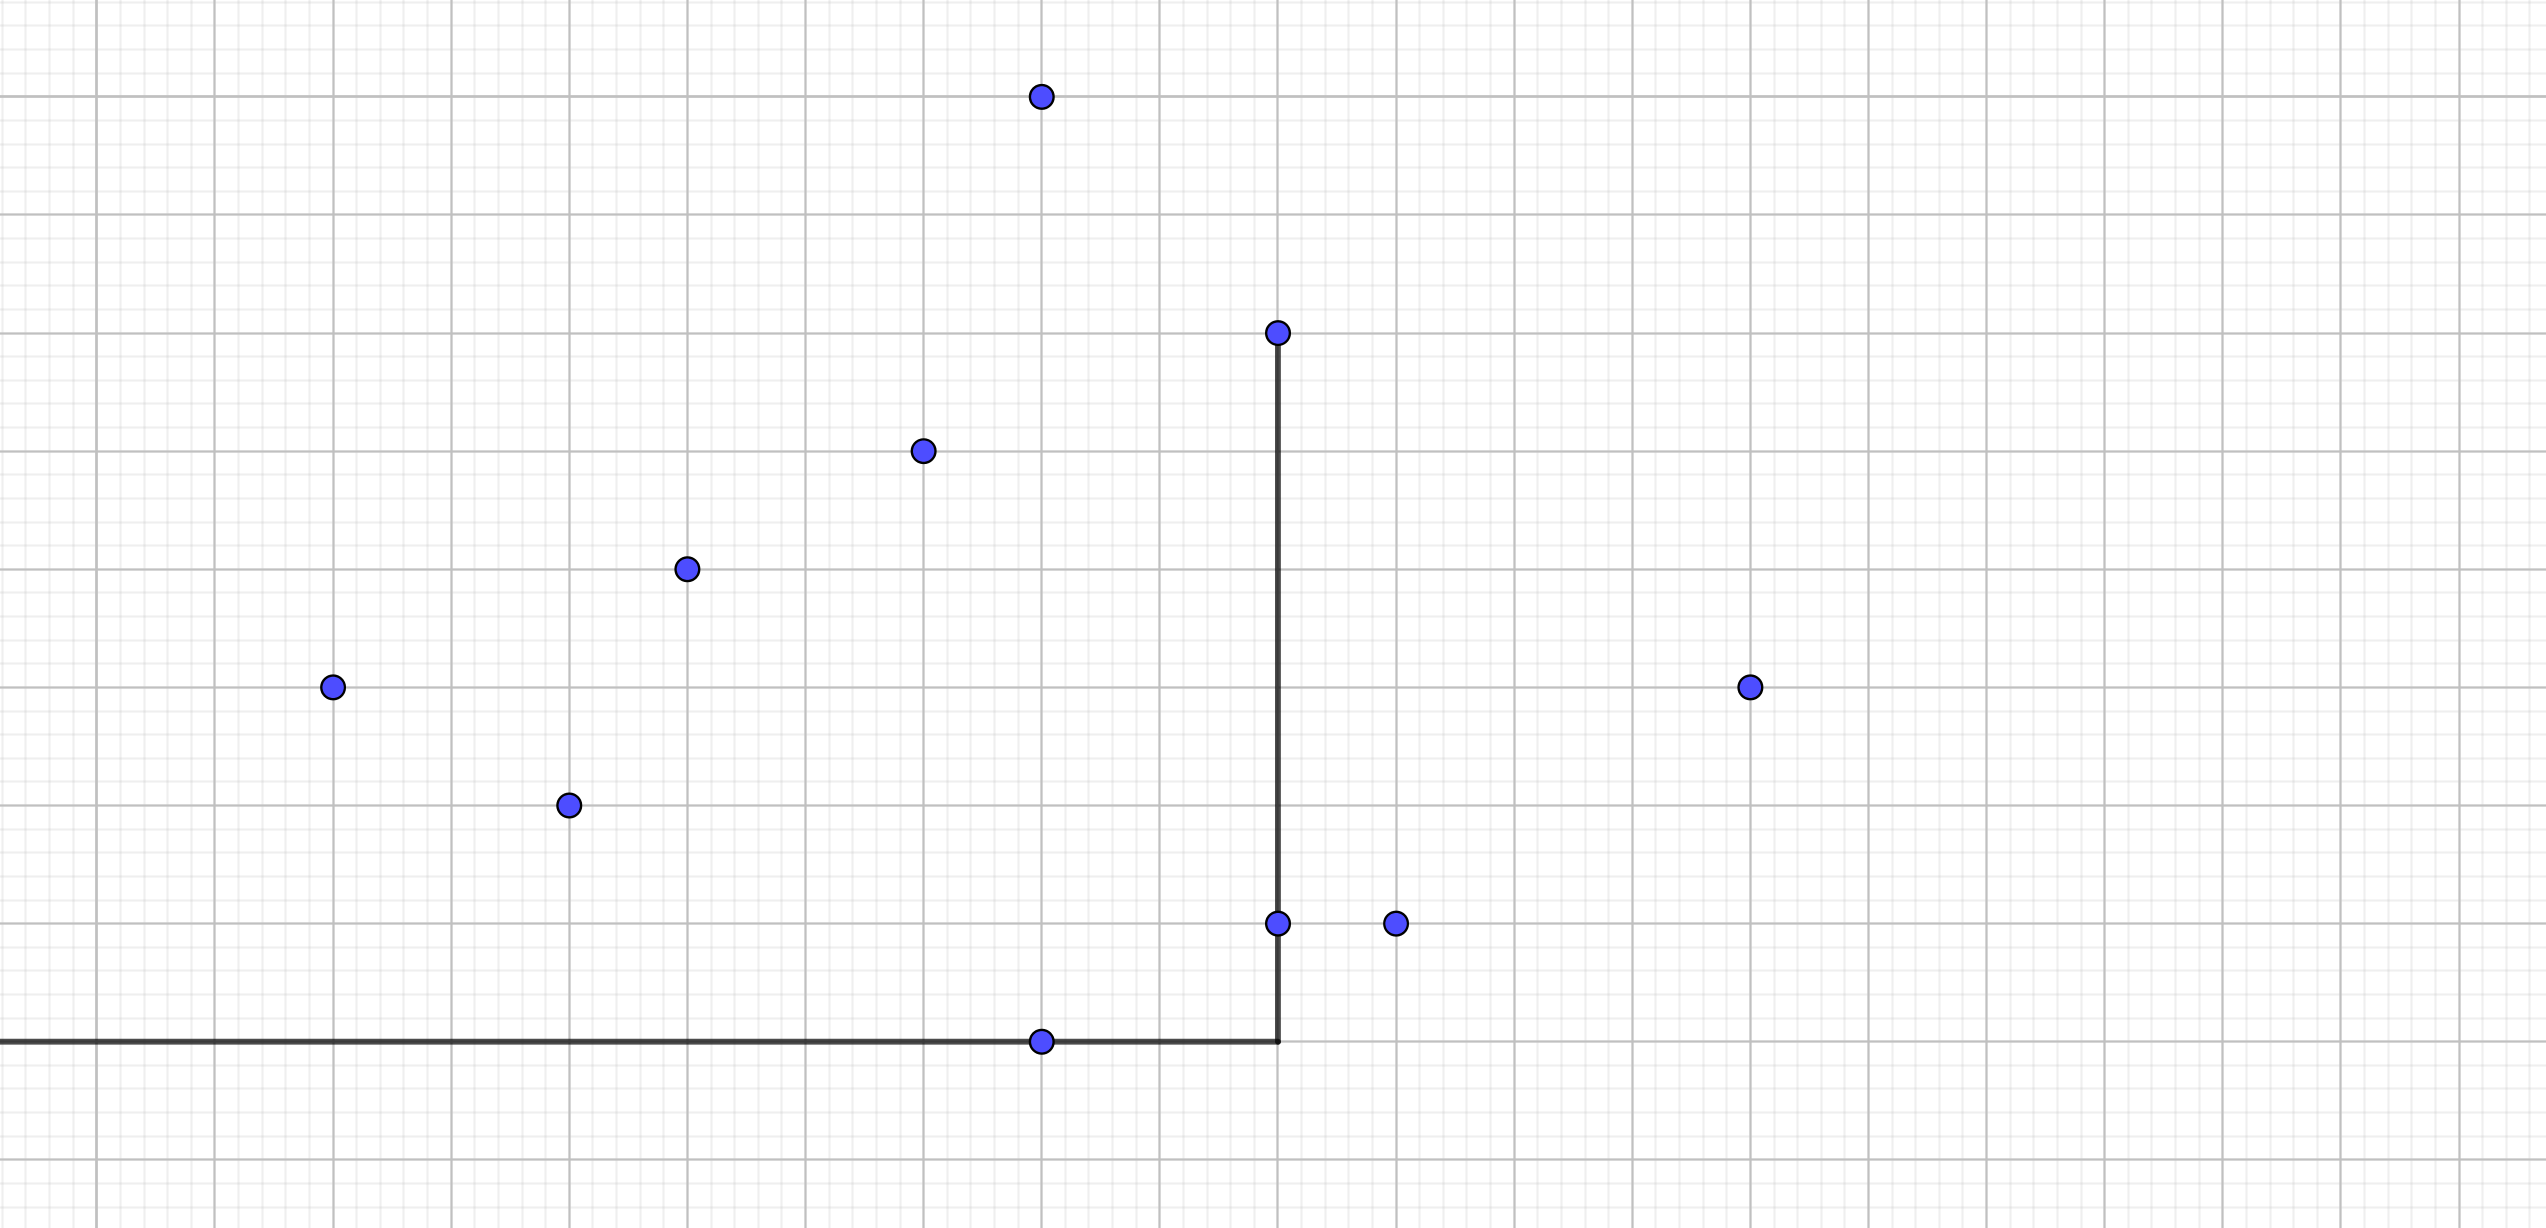
\includegraphics[width=\textwidth]{Prueba-misma-vertical-3}
\end{figure}
\end{frame}
\begin{frame}
\begin{block}{Teorema 1}
Sean $R$ y $B$ dos conjuntos ajenos de puntos rojos y azules tales que $R\cup B$ estan en posición general. Sea $\tau\left( R, B \right)$ el número de aristas $xy$ en el cierre convexo de $(R\cup B)$ tal que uno de $\lbrace x,y \rbrace$ es rojo y el otro es azul. Entonces el número de cruces en $T_{R} \cup T_{B}$ está dado por $$max\left\lbrace \frac{\tau(R, B)}{2}, 0 \right\rbrace$$.
\end{block}
\end{frame}
\begin{frame}
$\tau(R,B)= 6$
\begin{figure}[h]
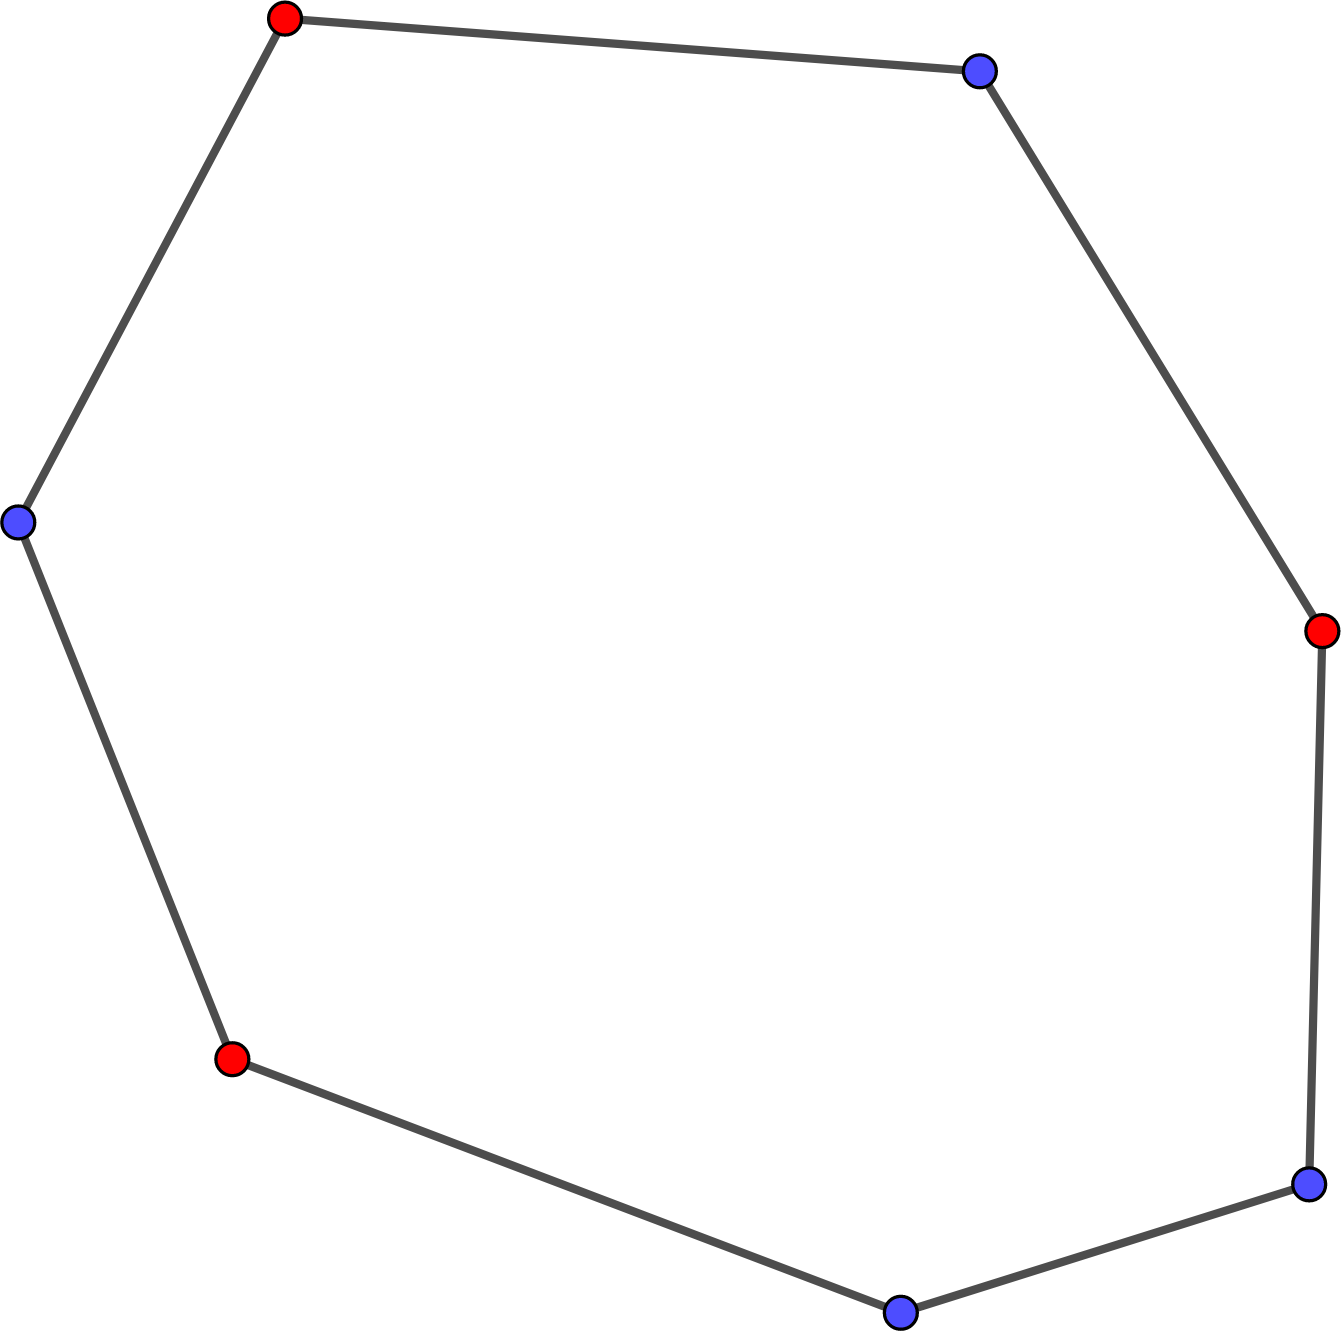
\includegraphics[width=5cm, height=5cm]{tauDeRyB}
\end{figure}
\end{frame}
\begin{frame}
\begin{figure}[h]
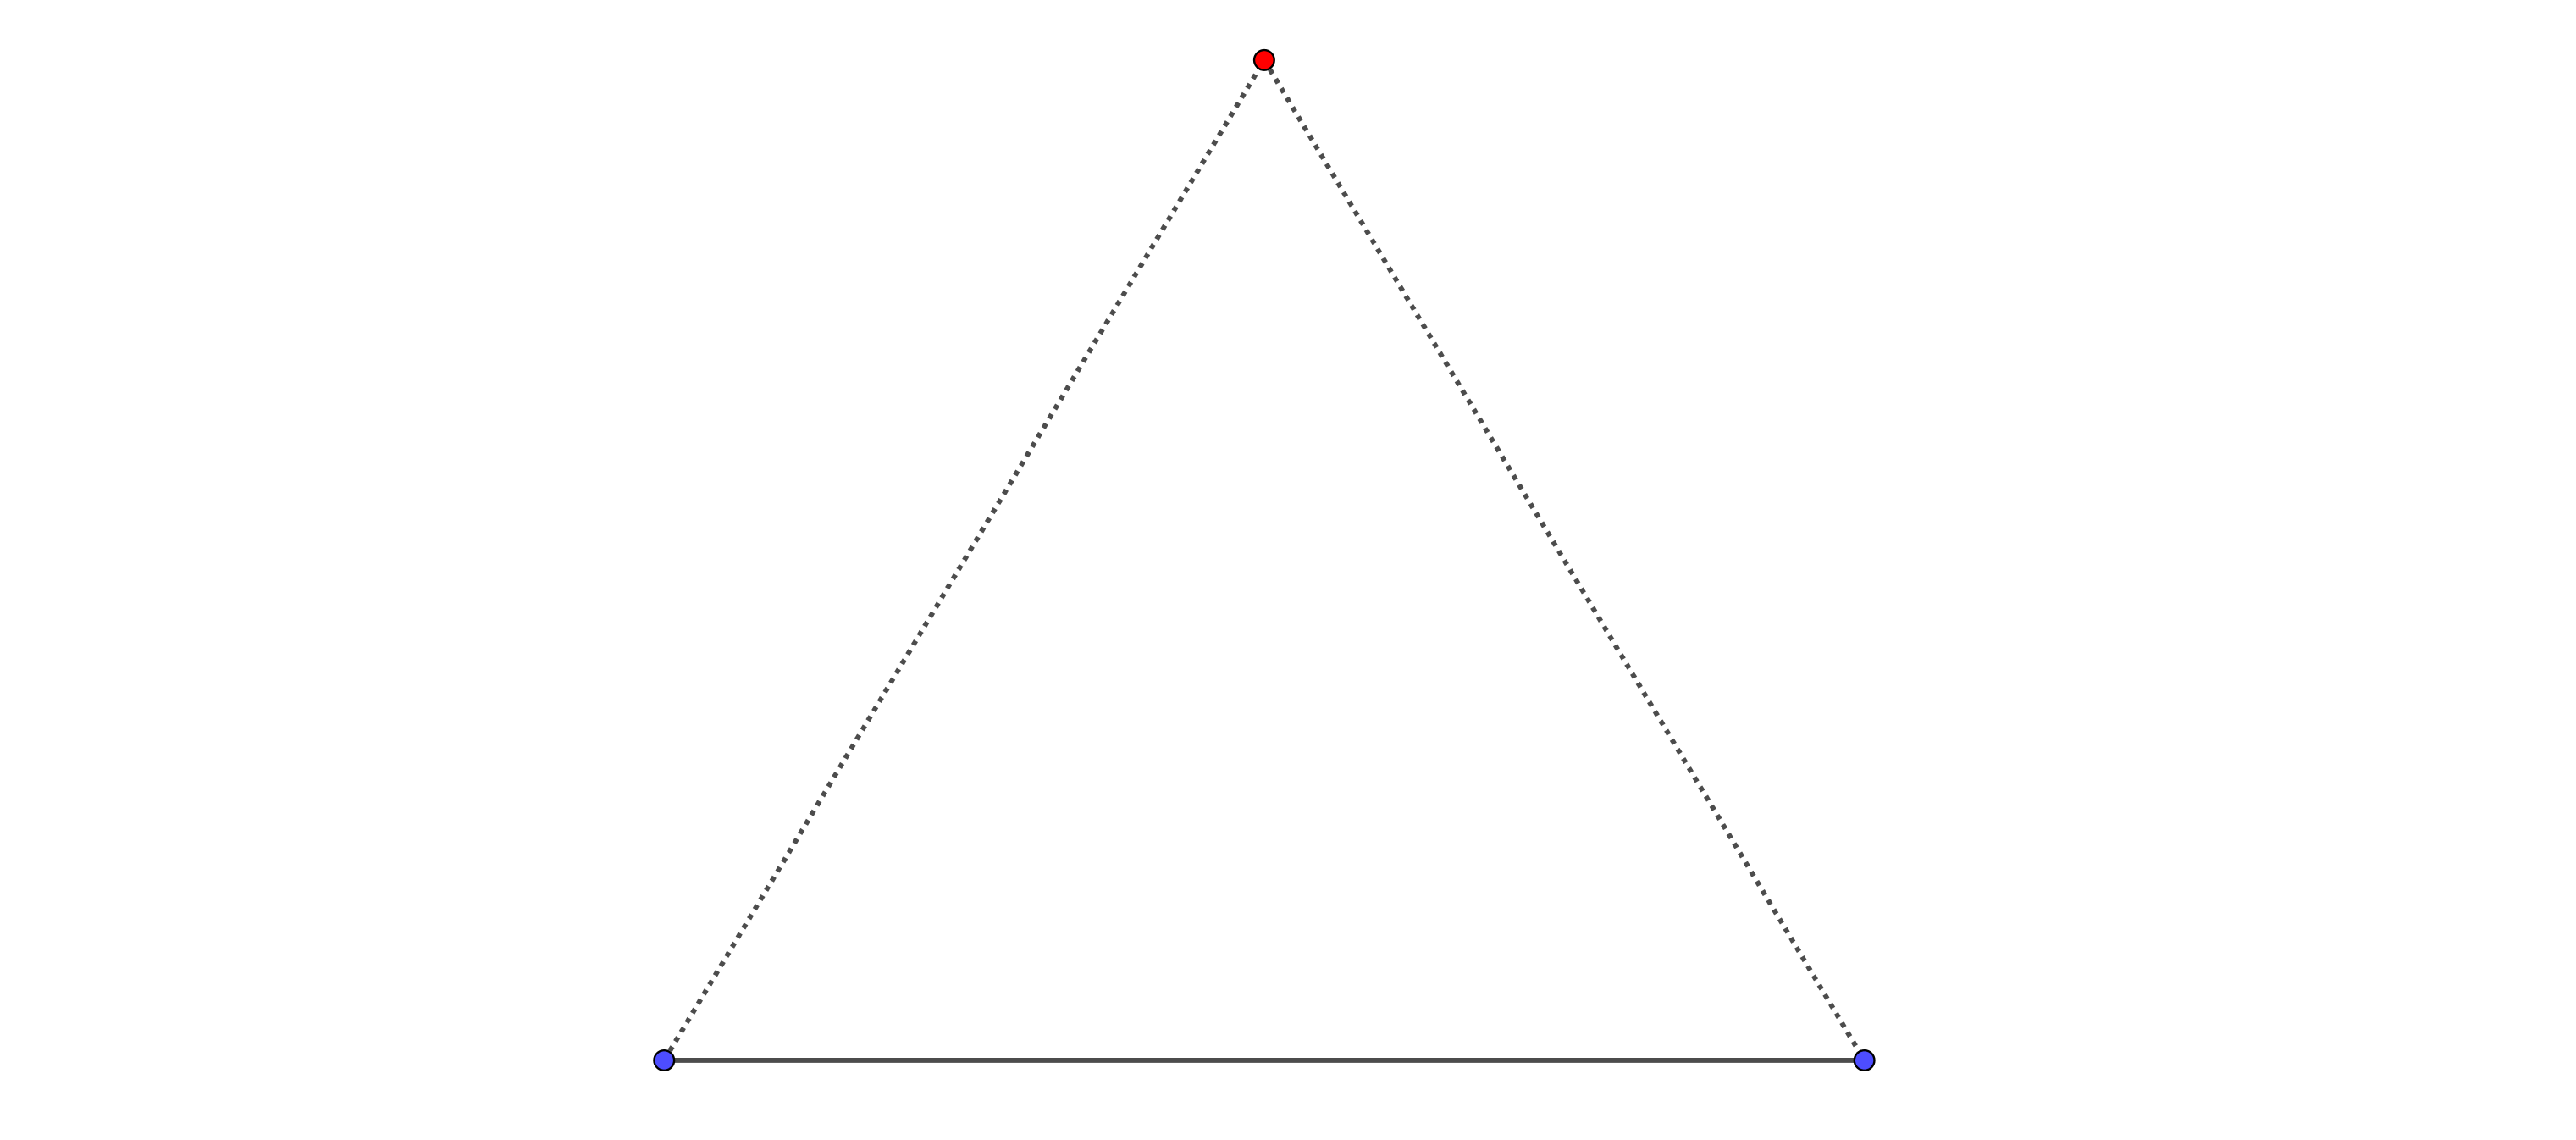
\includegraphics[width=\textwidth]{Tokunaga}
\end{figure}
\end{frame}
\begin{frame}
\begin{figure}[h]
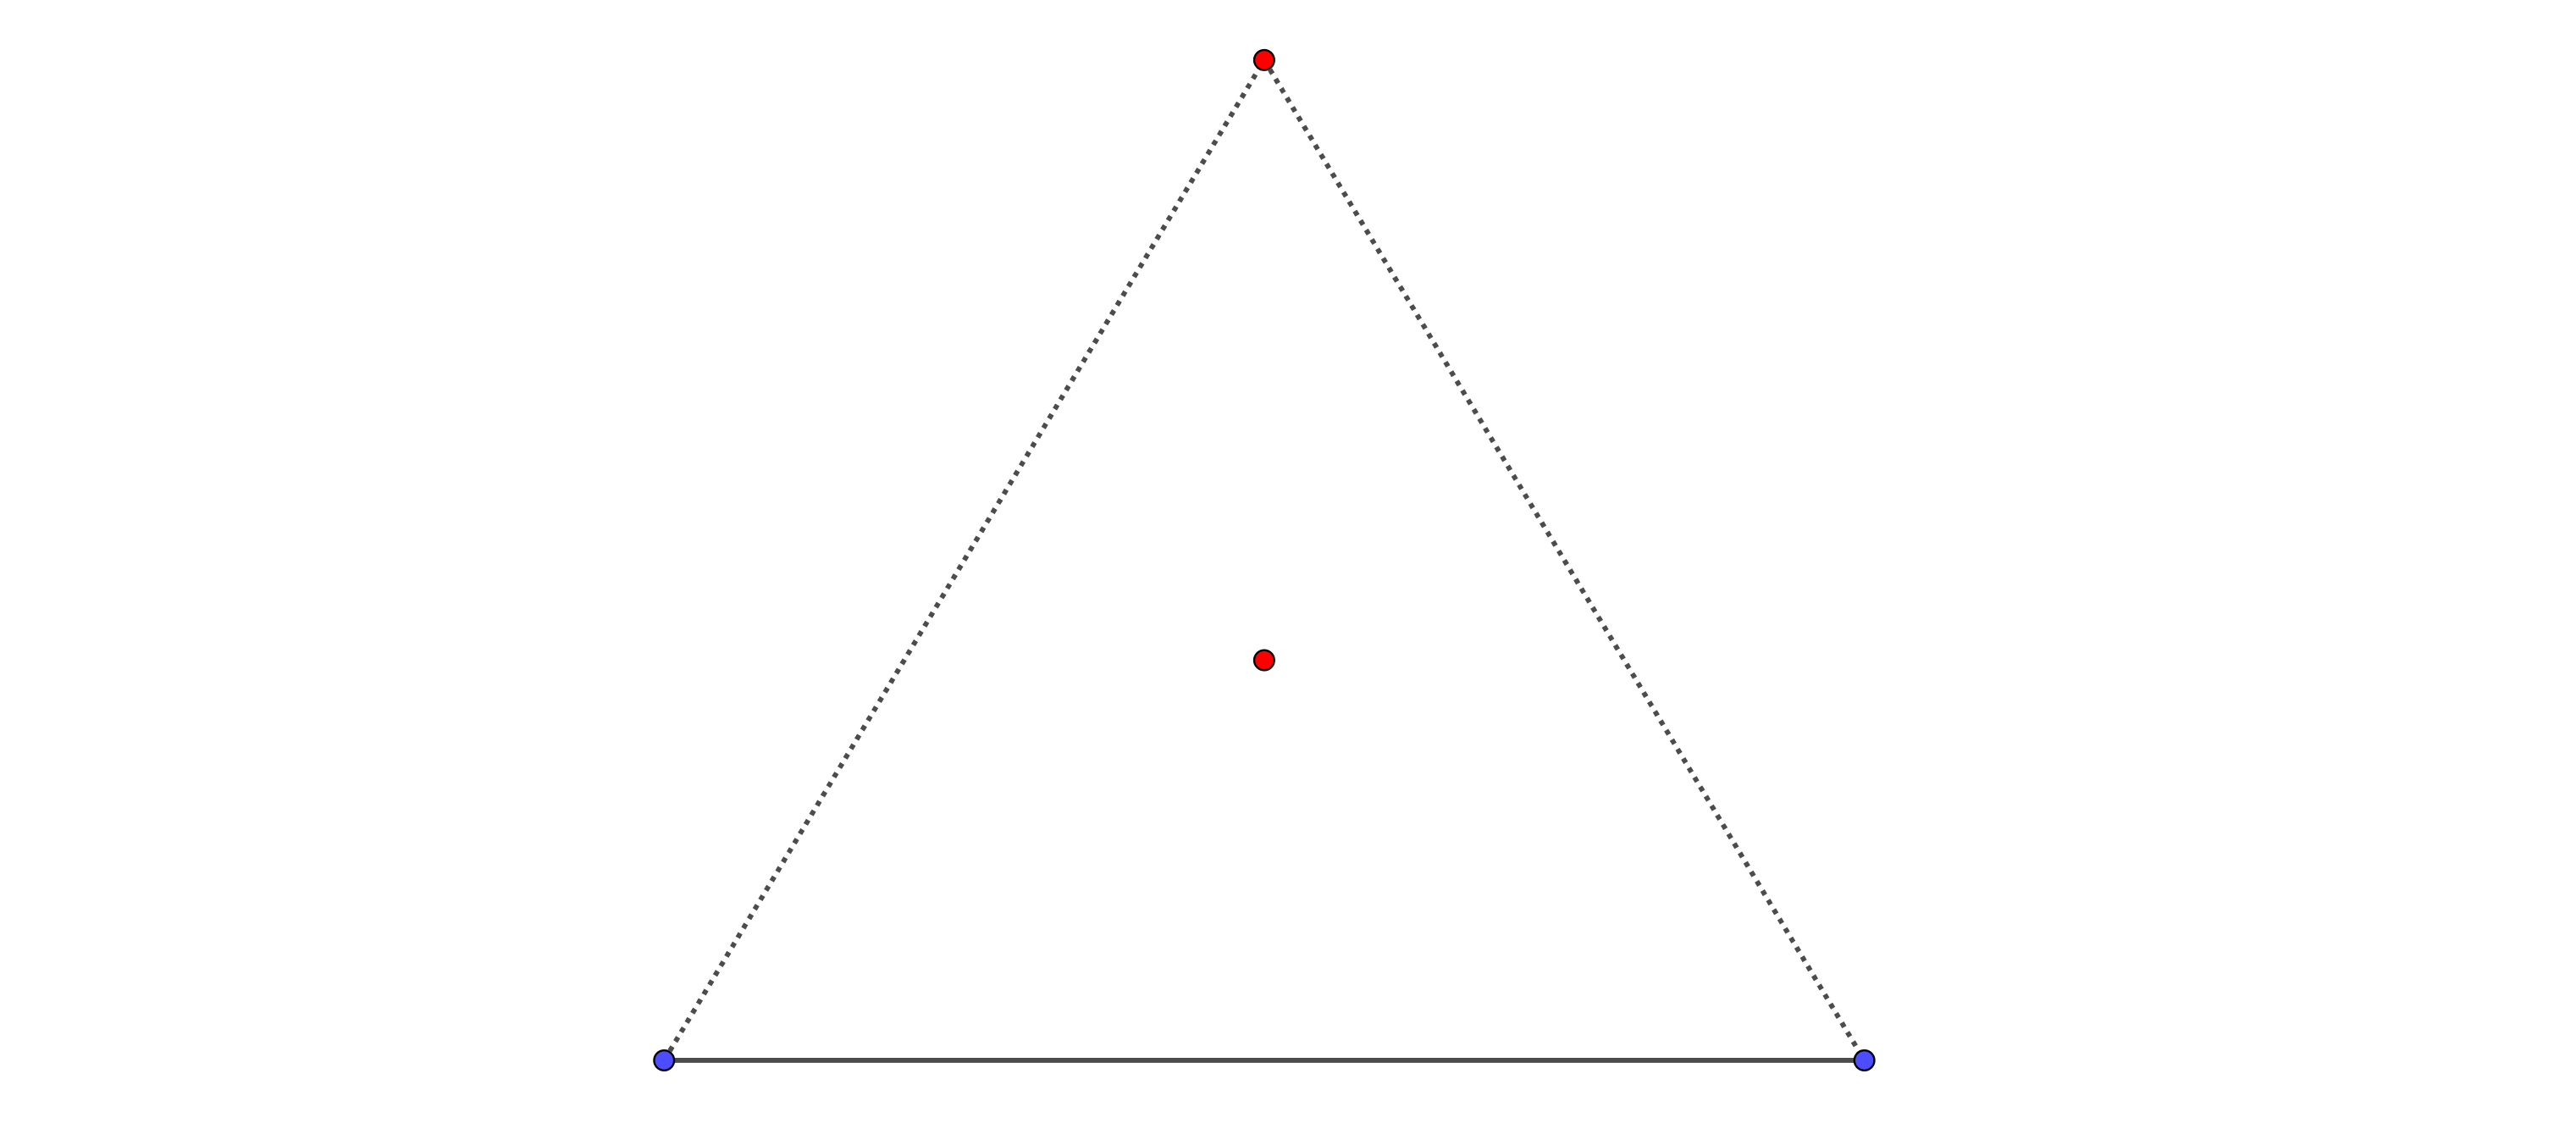
\includegraphics[width=\textwidth]{Tokunaga-2}
\end{figure}
\end{frame}
\begin{frame}
\begin{figure}[h]
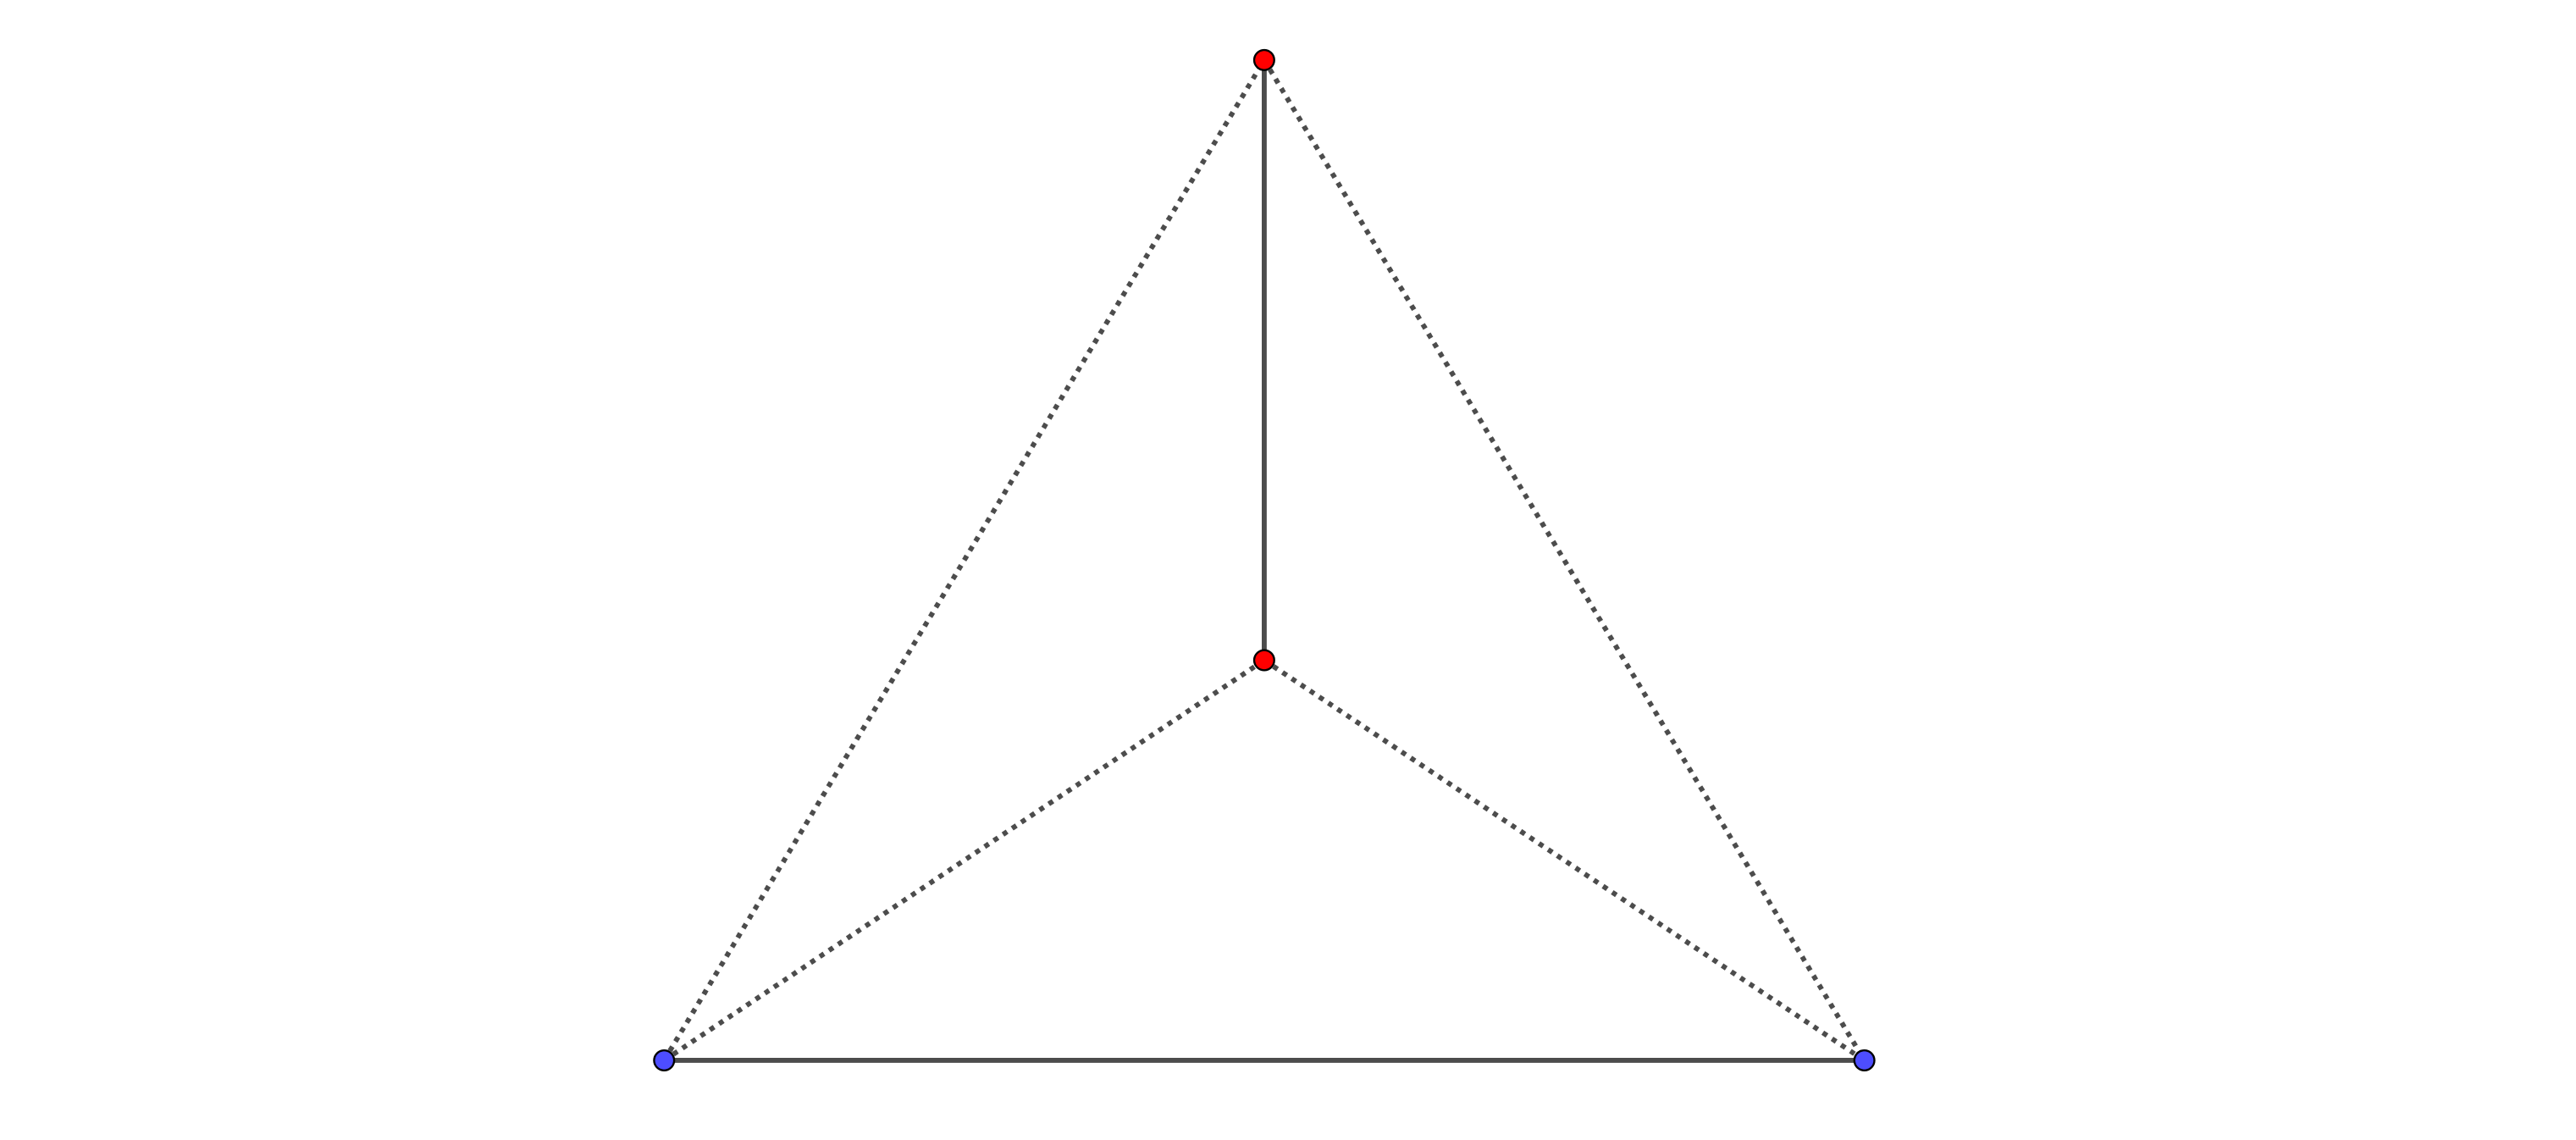
\includegraphics[width=\textwidth]{Tokunaga-3}
\end{figure}
\end{frame}
\begin{frame}
\begin{figure}[h]
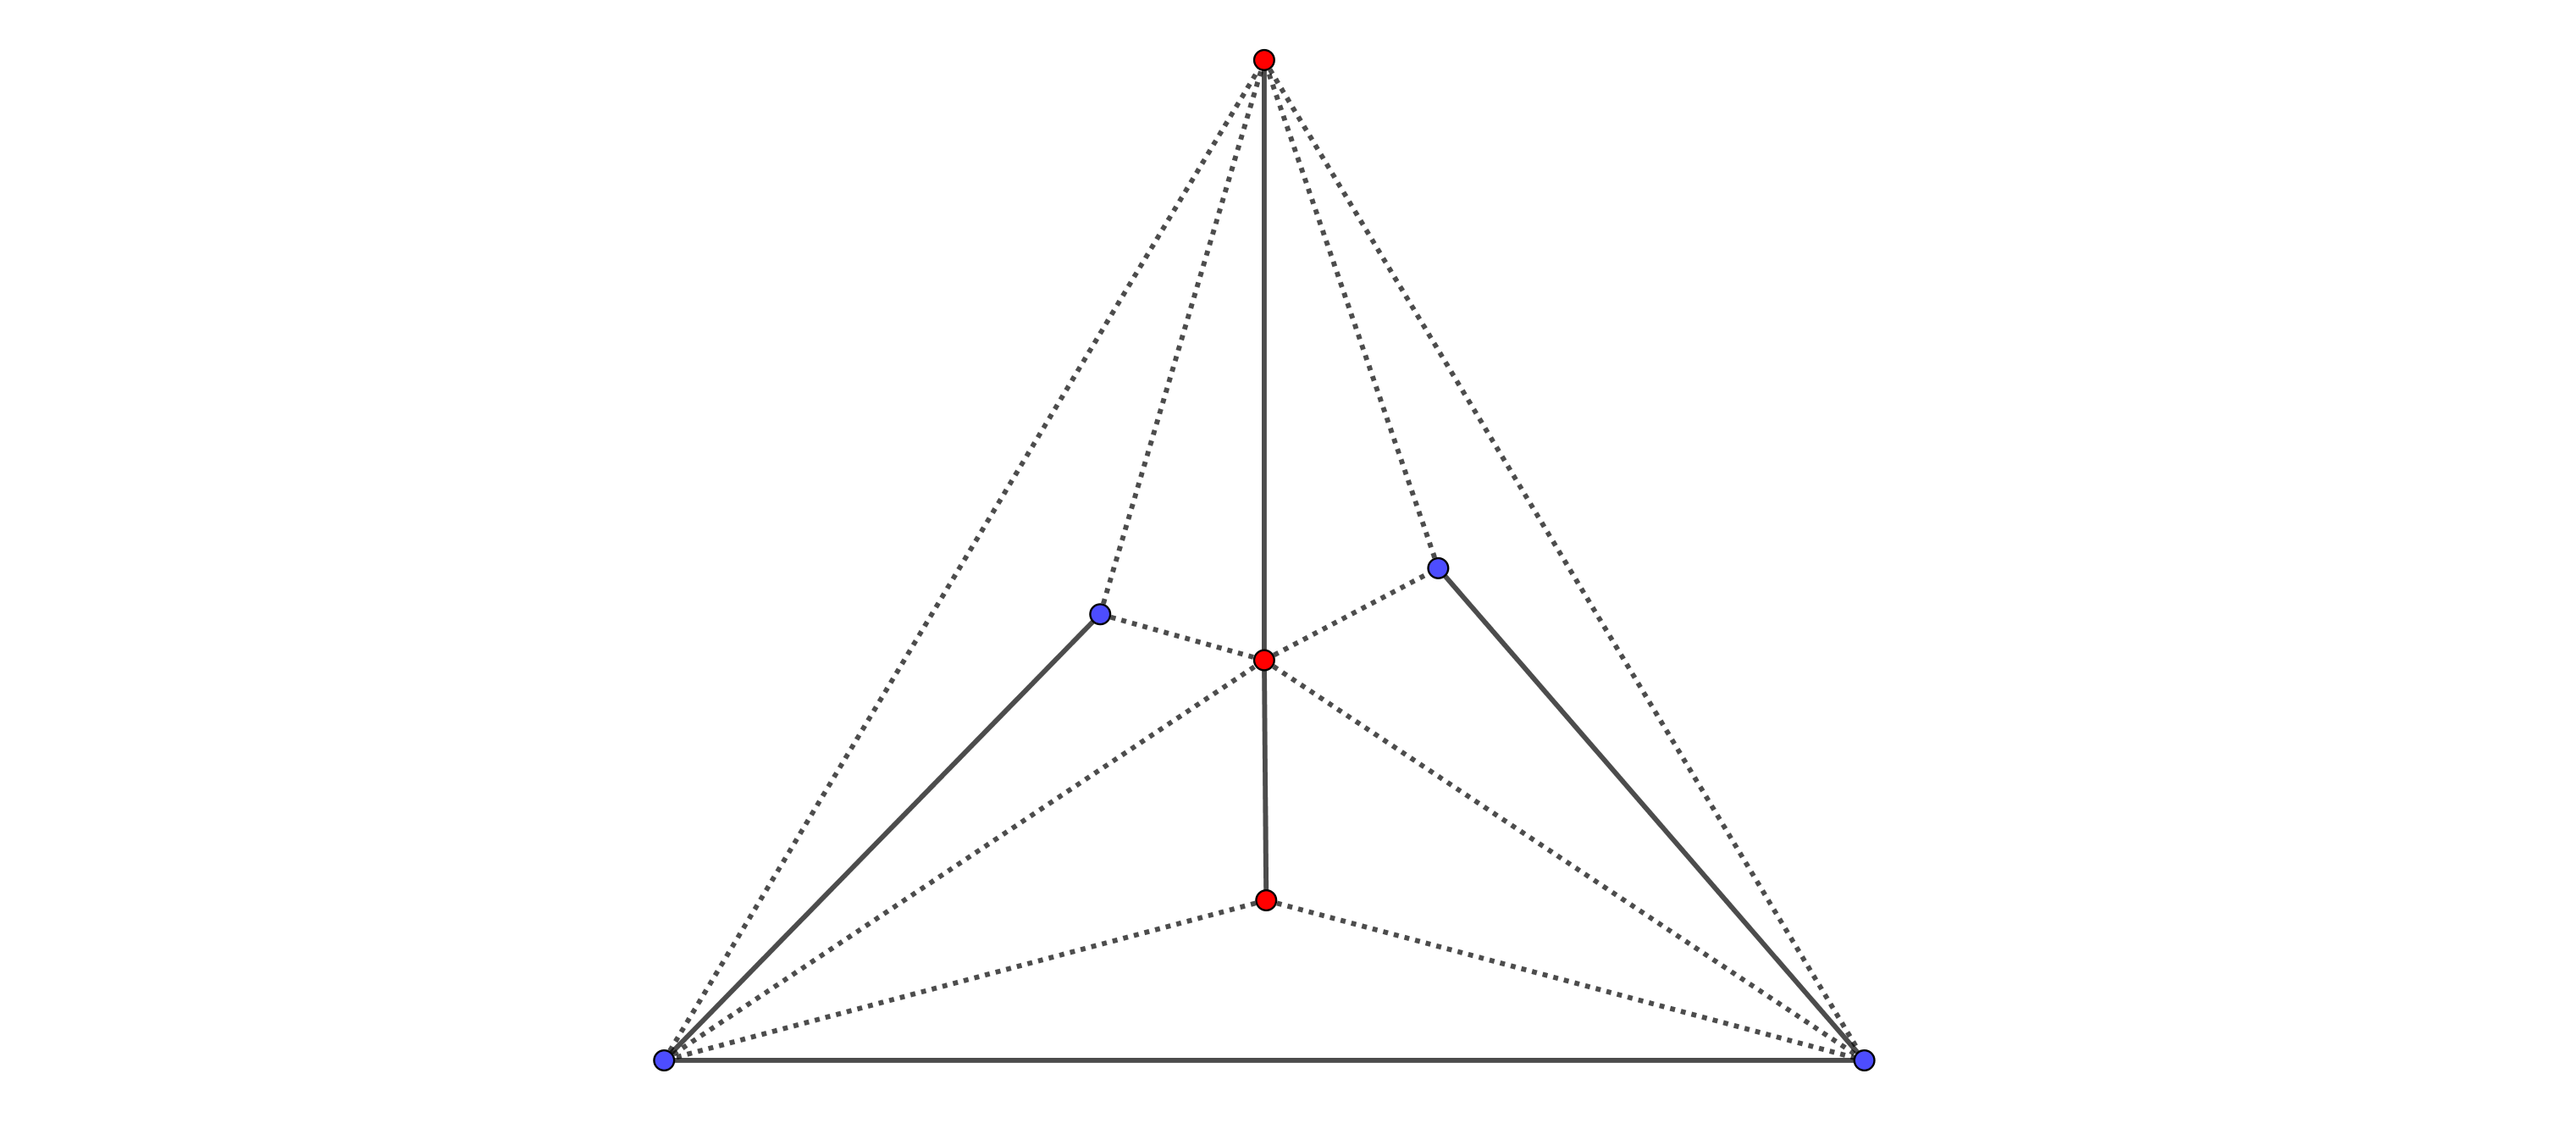
\includegraphics[width=\textwidth]{Tokunaga-4}
\end{figure}
\end{frame}
\begin{frame}
\begin{figure}[h]
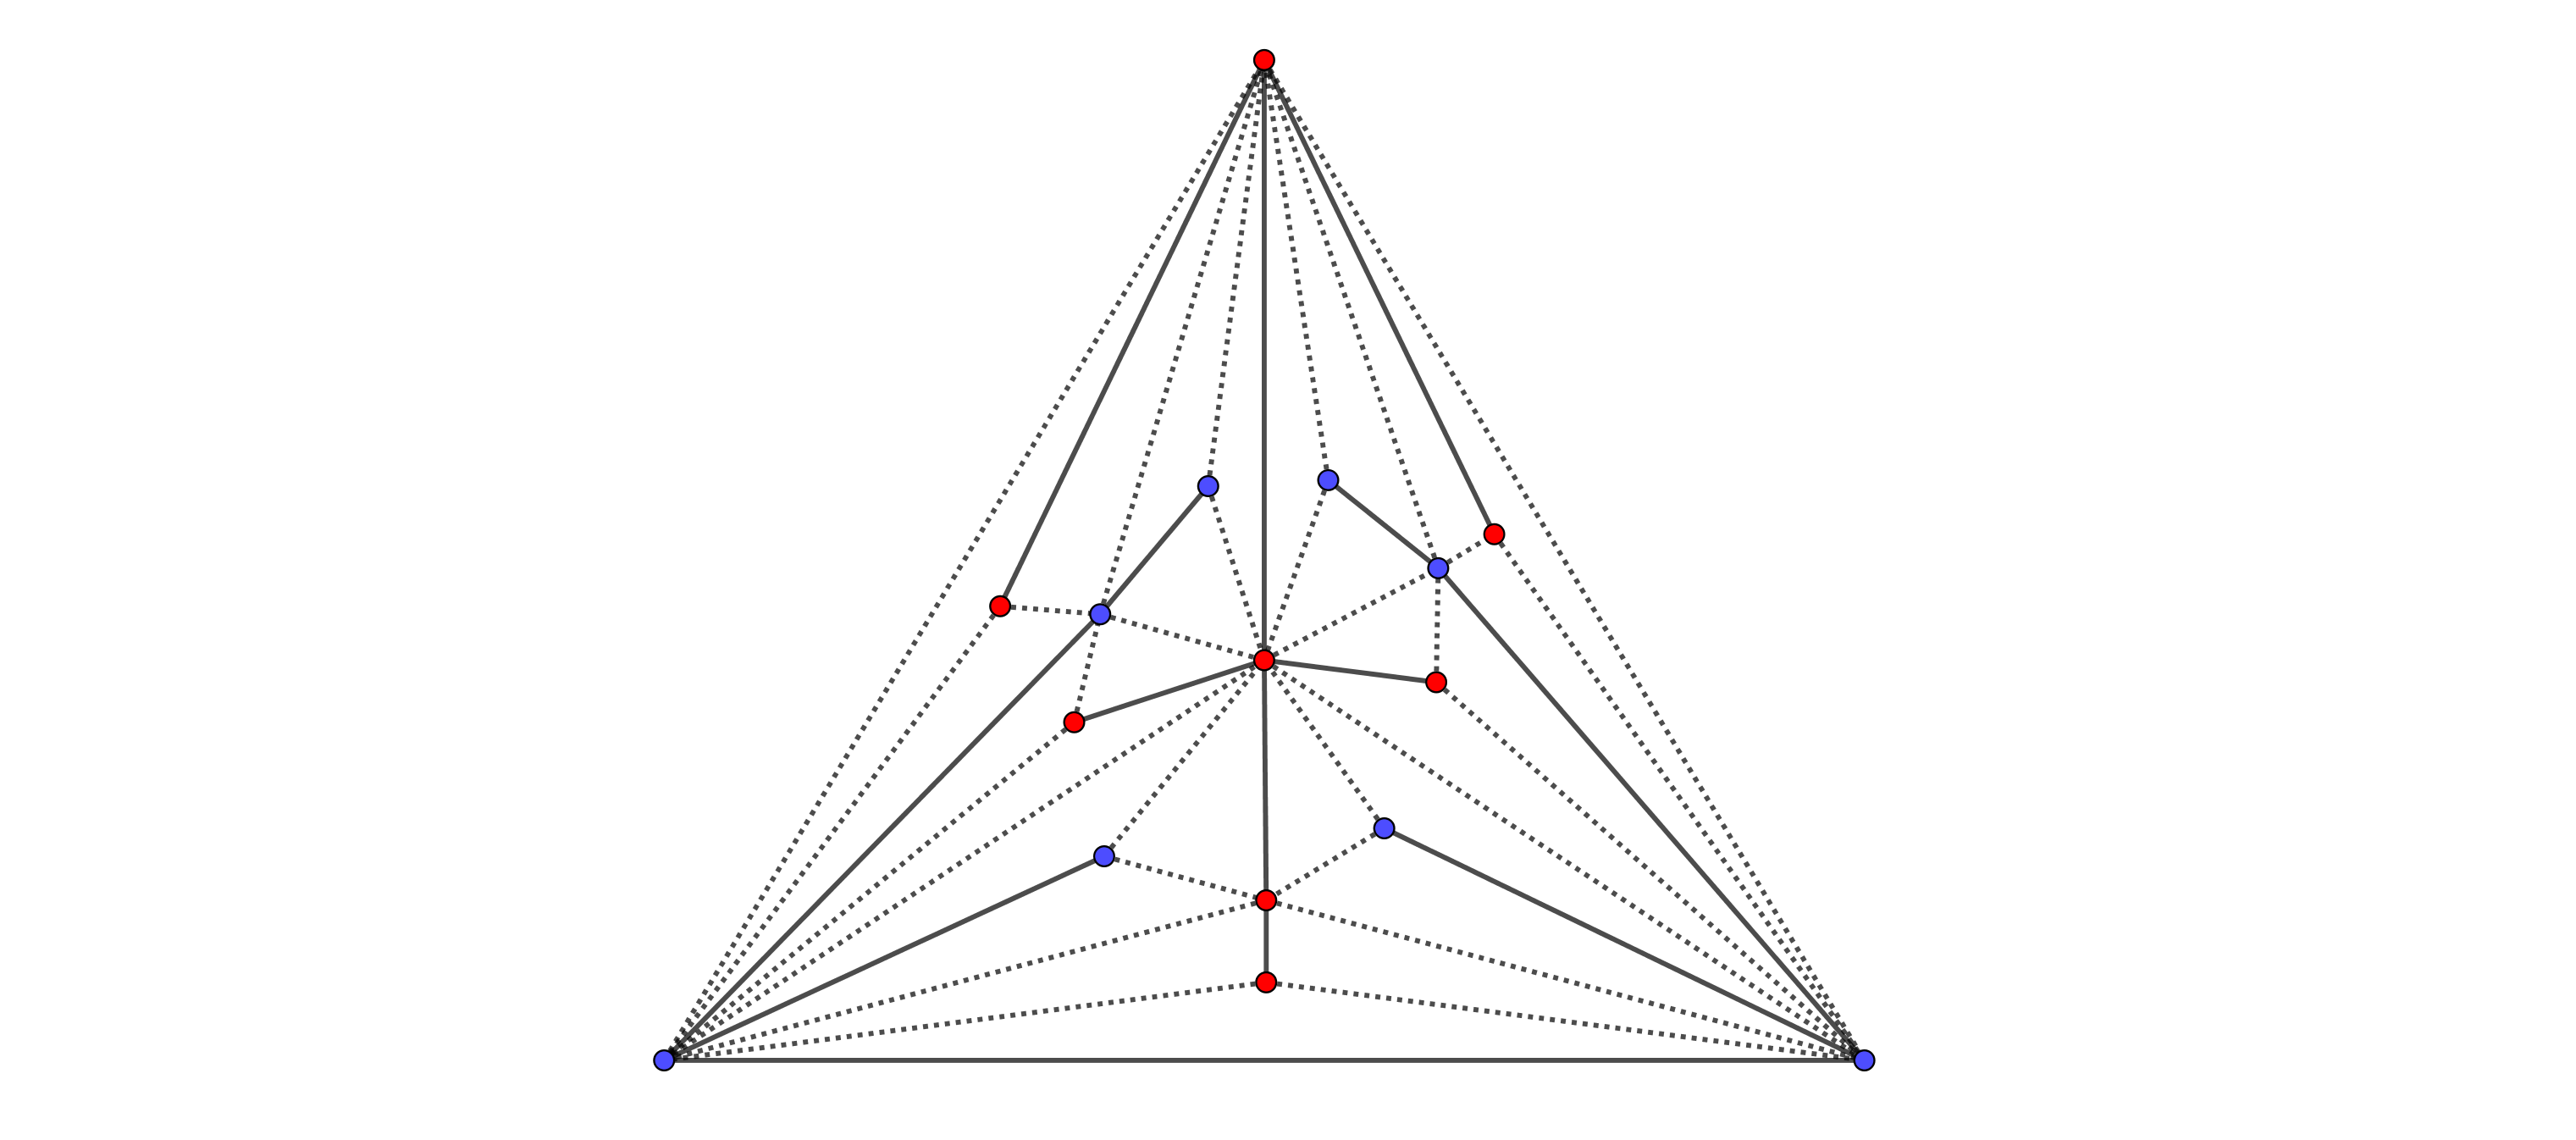
\includegraphics[width=\textwidth]{Tokunaga-5}
\end{figure}
\end{frame}
\begin{frame}
\begin{figure}[h]
\includegraphics[width=\textwidth]{Ejemplo-X-arbol}
\end{figure}
\end{frame}
\begin{frame}
\begin{figure}[h]
\includegraphics[width=\textwidth]{Ejemplo-X-arbol-2}
\end{figure}
\end{frame}
\begin{frame}
\begin{figure}[h]
$rect(S)$
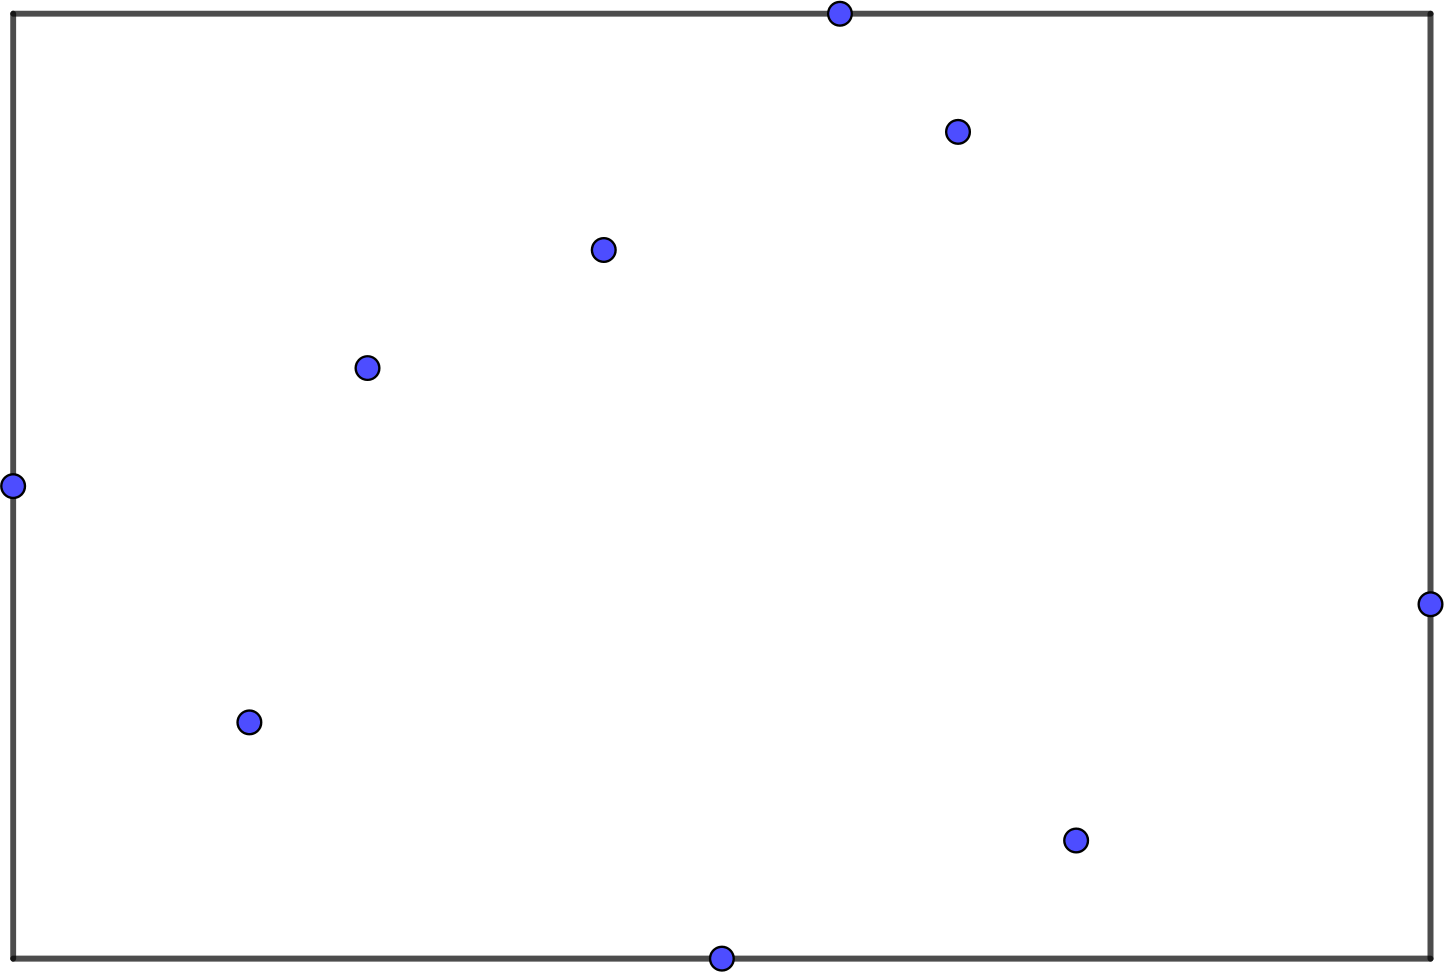
\includegraphics[width=\textwidth]{Ejemplo-rect-S}
\end{figure}
\end{frame}
\begin{frame}
\begin{figure}[h]
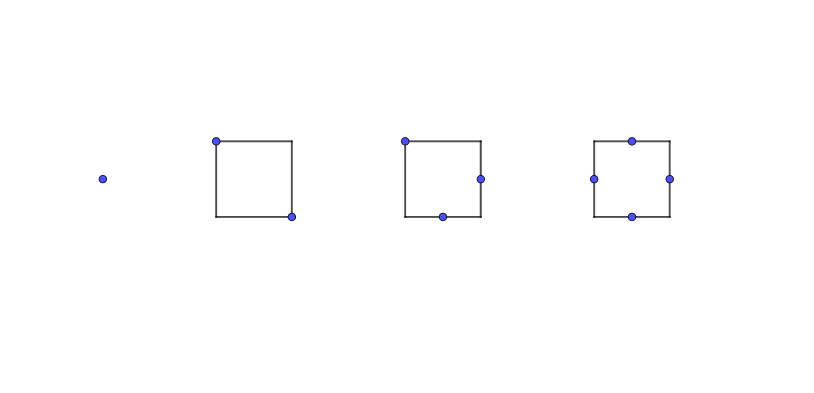
\includegraphics[width=\textwidth]{Cantidad-en-rect-S}
\end{figure}
\end{frame}
\begin{frame}
\begin{block}{Teorema 2}
Sean $R$ y $B$ conjuntos ajenos de puntos en el plano lattice, $R \cup B$ en posición general. Sea $\tau^*(R, B)$  el número de segmentos  $xy$ de L-líneas en la frontera de $rect(R\cup B)$  tal que uno de $\{ x,y\}$ es rojo y el otro es azul. Entonces $\tau^*(R, B)$  es 0, 2 o 4 y el máximo número de cruces entre $T_R$ y $T_B$ es 1 cuando $\tau^*(R, B) = 4$. Además si $\tau^*(R, B) \leq 2$ podemos dibujar los árboles sin cruces con $\Delta(T_R) \leq 3$ y $\Delta(T_B) \leq 3$. \cite{Kano2013}
\end{block}
\end{frame}
\begin{frame}
\begin{figure}[h]
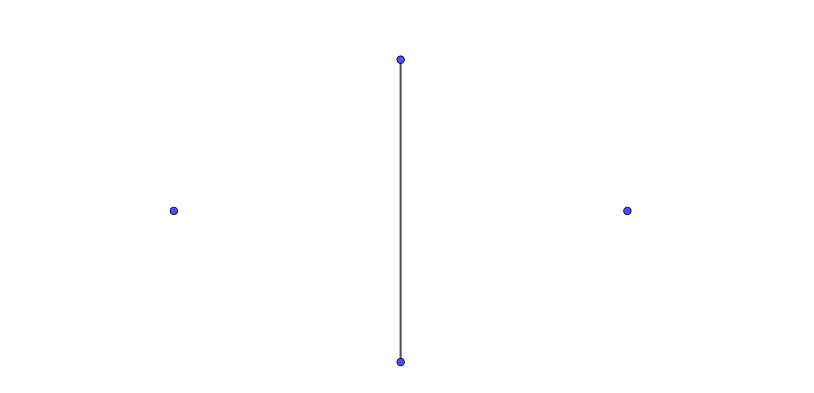
\includegraphics[width=\textwidth]{Arbol-imposible-sin-cruces}
\end{figure}
\end{frame}
\begin{frame}
\begin{block}{Polígono espiral ortogonal}
Un polígono espiral ortogonal es un polígono cuya frontera consiste de dos cadenas de aristas llamadas interna y externa. Cada ángulo interno de la cadena exterior es de $\frac{\pi }{2}$ y cada ángulo externo de la cadena interna es de $\frac{3\pi }{2}$.
\end{block}
\end{frame}
\begin{frame}
\begin{figure}[h]
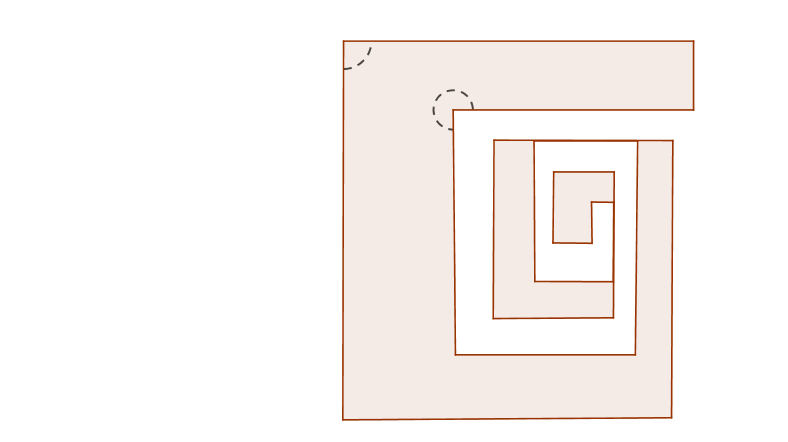
\includegraphics[width=\textwidth]{Poligono-espiral}
\end{figure}
\end{frame}
\begin{frame}
\begin{block}{Lema 1}
Sea $P$ un polígono espiral ortogonal en el plano lattice y $S$ un conjunto de puntos en posición general contenido en $P$ y asumamos que cada arista de la cadena exterior tiene exactamente un punto y la cadena interior tambien tiene exactamente un punto o esta incluida en alguna cadena exterior. Entonces existe un arbol generador $T$  tal que $\Delta (T) \leq 3$ y $T$ está dentro de $P$.
\end{block}
\end{frame}
\begin{frame}
\begin{figure}[h]
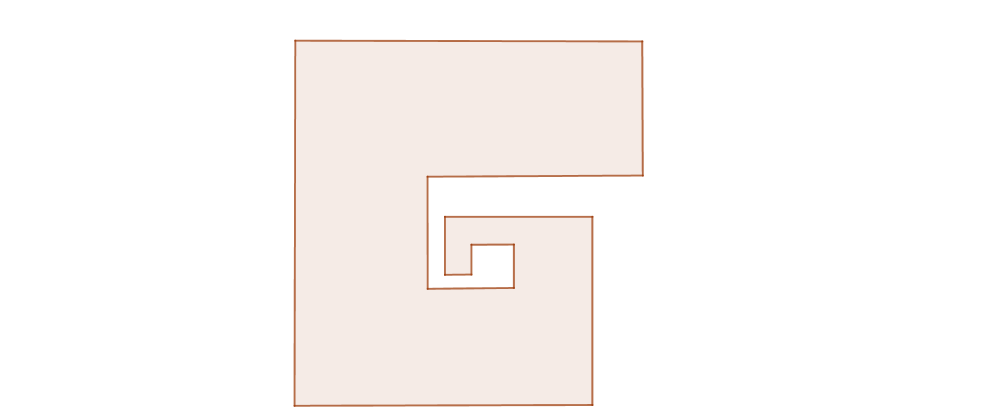
\includegraphics[width=\textwidth]{Poligono-sin-planos}
\end{figure}
\end{frame}
\begin{frame}
\begin{figure}[h]
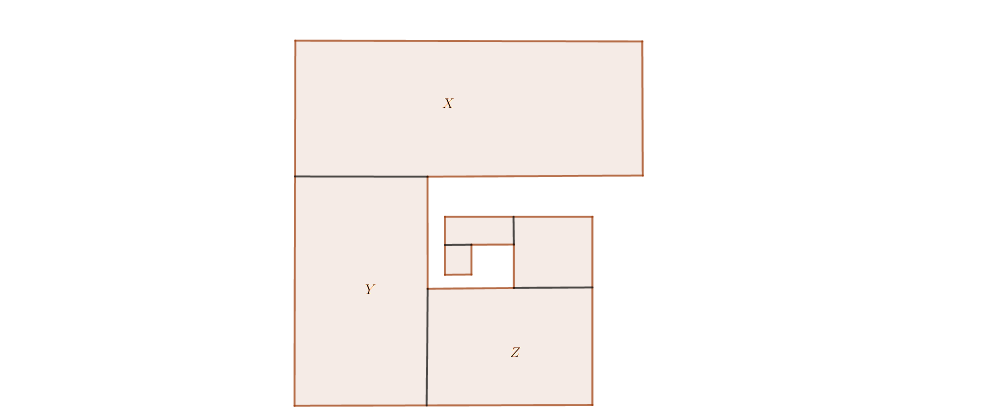
\includegraphics[width=\textwidth]{Poligono-sin-planos-2}
\end{figure}
\end{frame}
\begin{frame}
\begin{figure}[h]
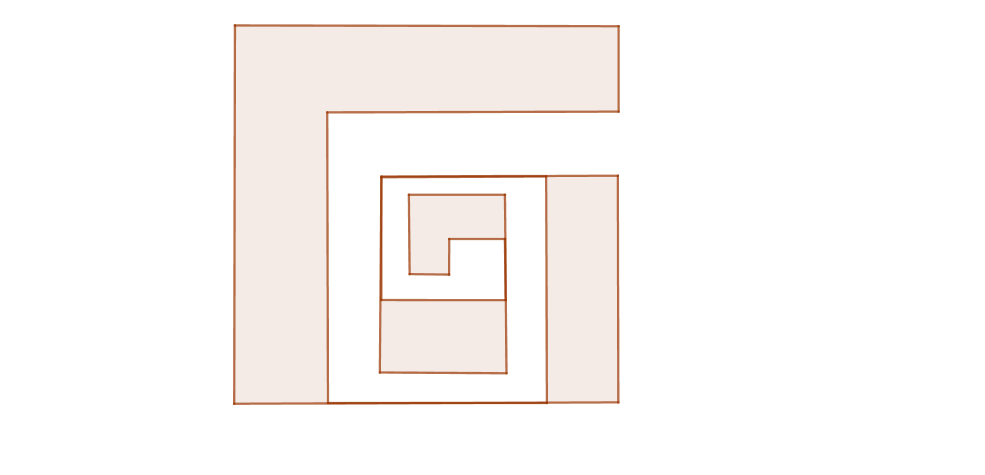
\includegraphics[width=\textwidth]{Poligono-con-planos}
\end{figure}
\end{frame}
\begin{frame}
\begin{figure}[h]
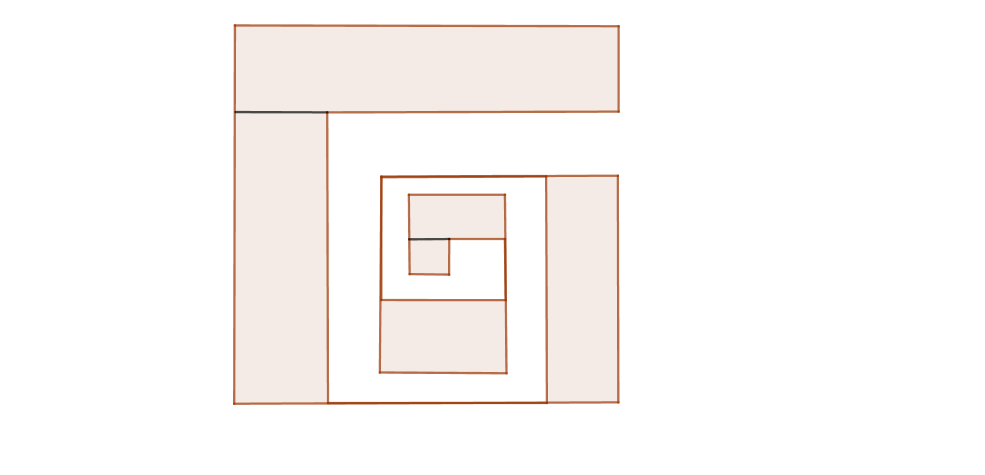
\includegraphics[width=\textwidth]{Poligono-con-planos-2}
\end{figure}
\end{frame}
\begin{frame}
\begin{figure}[h]
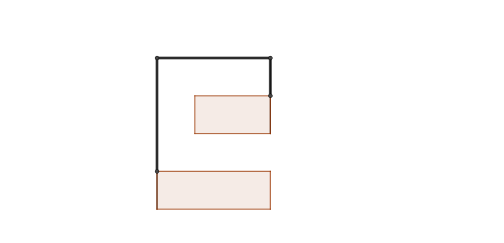
\includegraphics[width=\textwidth]{3-rectangulos-planos}
\end{figure}
\end{frame}
\begin{frame}
\begin{figure}[h]
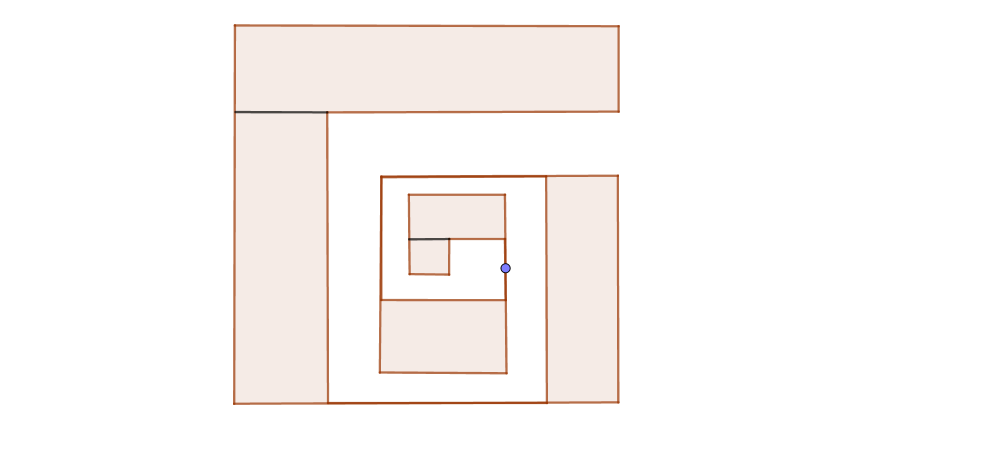
\includegraphics[width=\textwidth]{Poligono-con-planos-3}
\end{figure}
\end{frame}
\begin{frame}
\begin{figure}[h]
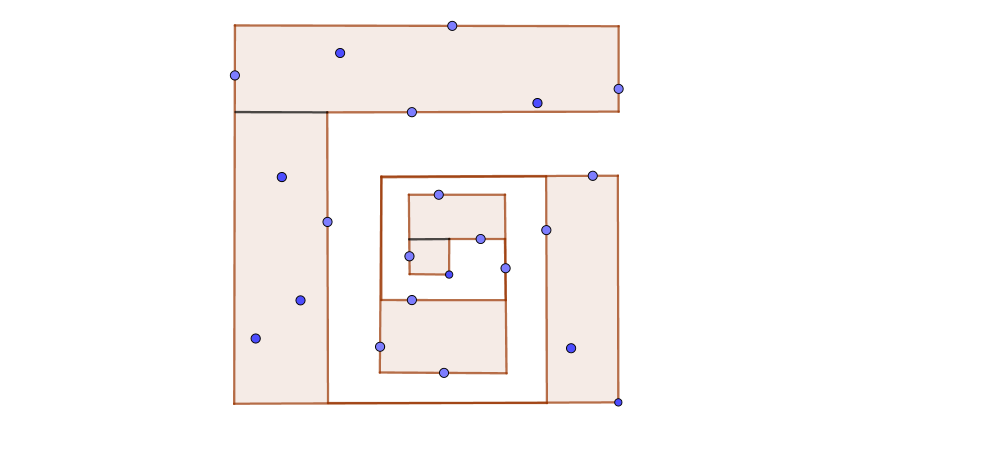
\includegraphics[width=\textwidth]{Poligono-con-planos-4}
\end{figure}
\end{frame}
\begin{frame}
\frametitle{Overview de las trayectorias}
Las trayectorias que construiremos en los  rectángulos no planos:

\begin{itemize}
 \item<1-> Comienzan en el punto superior y terminan en el inferior.
 \item<2-> Pasan por todos los puntos del rectángulo.
 \item<3> Cada segmento de  L-línea $xy$ tal que $x$ está arriba de $y$ empieza en $x$ hacia un lado y termina en $y$ por arriba.
\end{itemize}

\end{frame}
\begin{frame}
\begin{figure}[h]
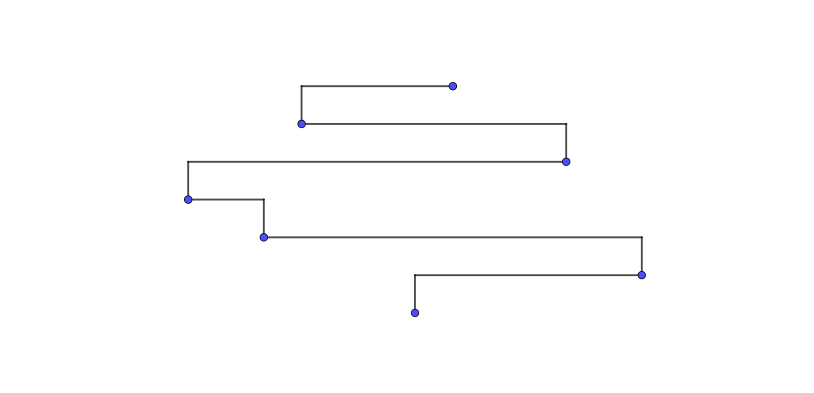
\includegraphics[width=\textwidth]{Trayectoria-monotona}
\end{figure}
\end{frame}
\begin{frame}
\begin{figure}[h]
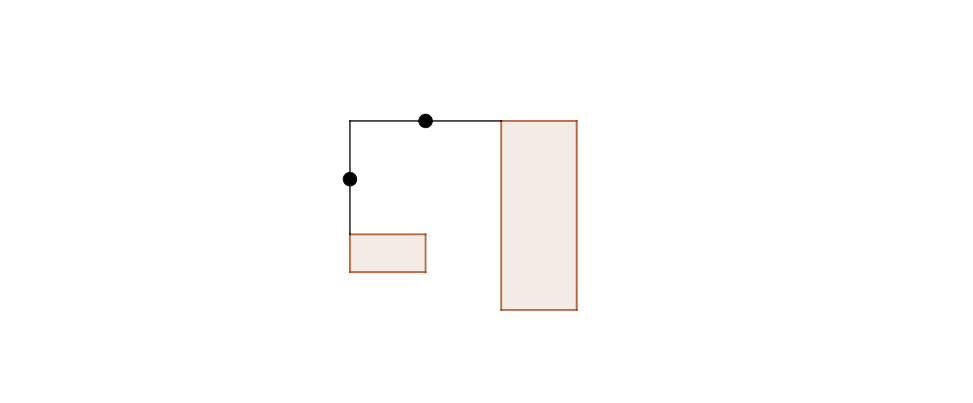
\includegraphics[width=\textwidth]{Dummy-point}
\end{figure}
\end{frame}
\begin{frame}
\begin{figure}[h]
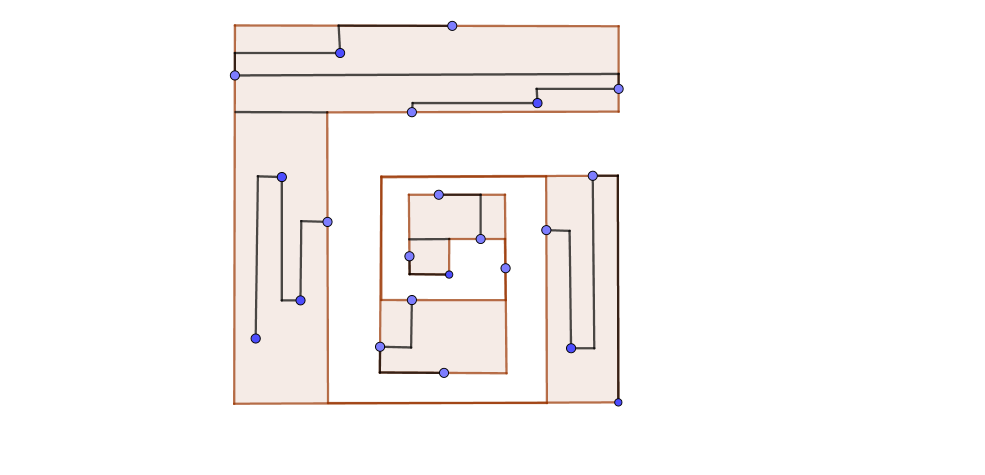
\includegraphics[width=\textwidth]{Poligono-con-planos-5}
\end{figure}
\end{frame}
\begin{frame}
\begin{figure}[h]
Caso 1. $Tr_{i+1} \neq \emptyset$
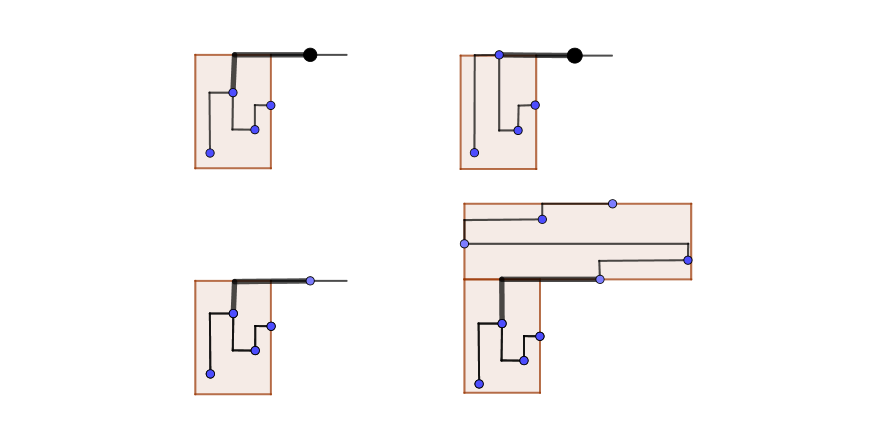
\includegraphics[width=\textwidth]{Caso-1}
\end{figure}
\end{frame}
\begin{frame}
\begin{figure}[h]
Caso 2. $Tr_{i+1} = \emptyset$
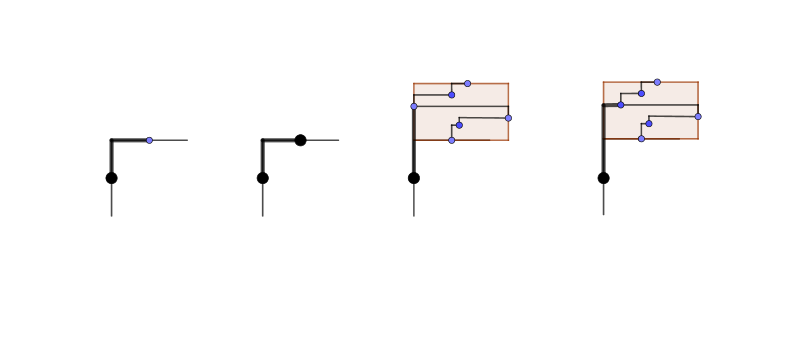
\includegraphics[width=\textwidth]{Caso-2}
\end{figure}
\end{frame}
\begin{frame}
\begin{figure}[h]
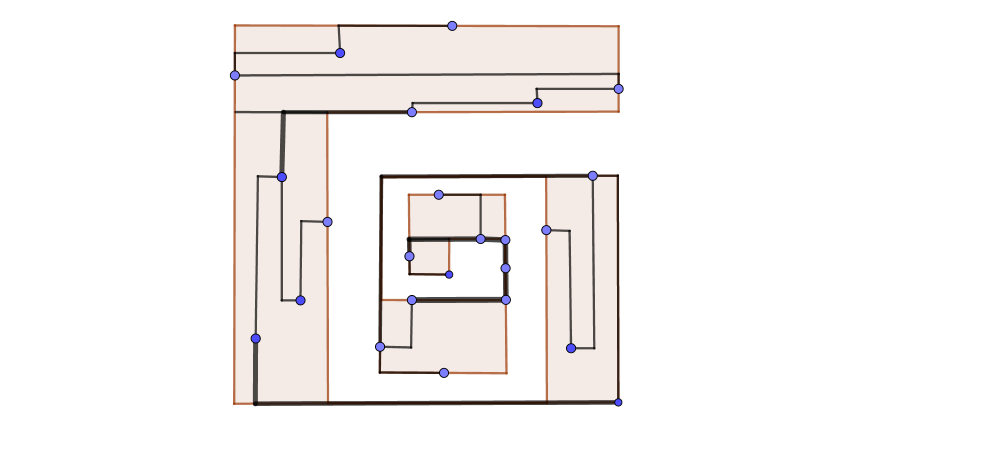
\includegraphics[width=\textwidth]{Poligono-con-planos-6}
\end{figure}
\end{frame}
\begin{frame}
El arbol que construimos cumple que:
\begin{enumerate}
\item $\Delta (T) \leq 3$
\item está contenido en el polígono espiral
\end{enumerate}
\end{frame}
\begin{frame}
\begin{figure}[h]
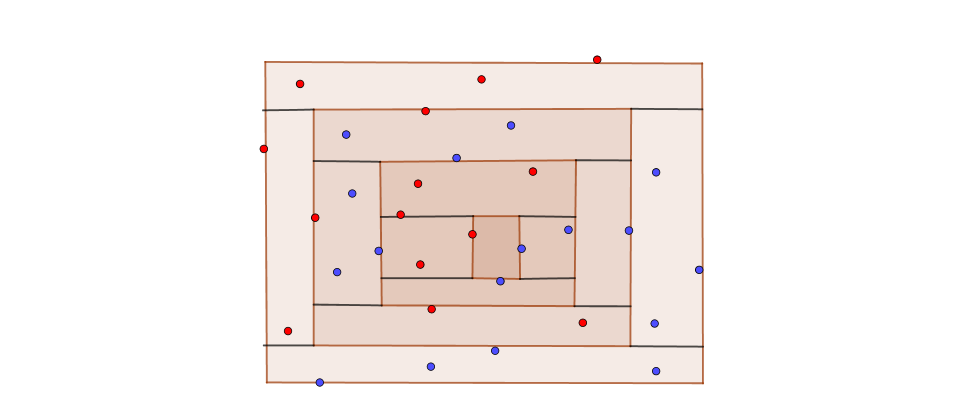
\includegraphics[width=\textwidth]{Construccion-poligono-2-alternancia}
\end{figure}
\end{frame}
\begin{frame}
\begin{figure}[h]
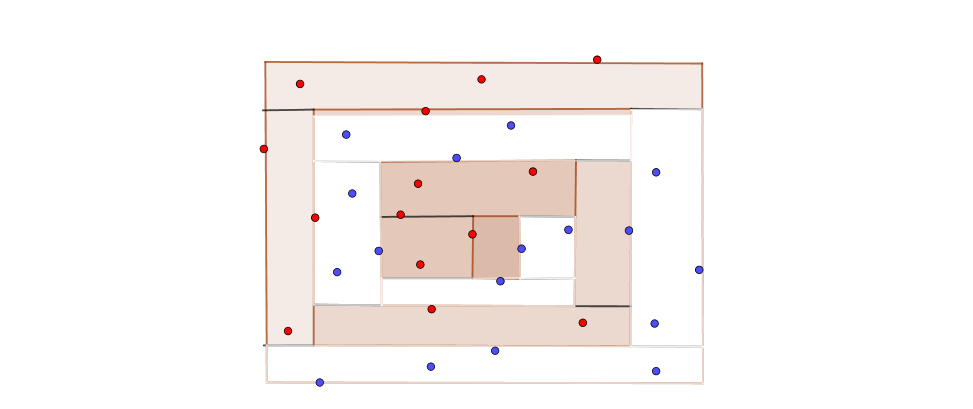
\includegraphics[width=\textwidth]{Construccion-poligono-2-alternancia-2}
\end{figure}
\end{frame}
\begin{frame}
\begin{figure}[h]
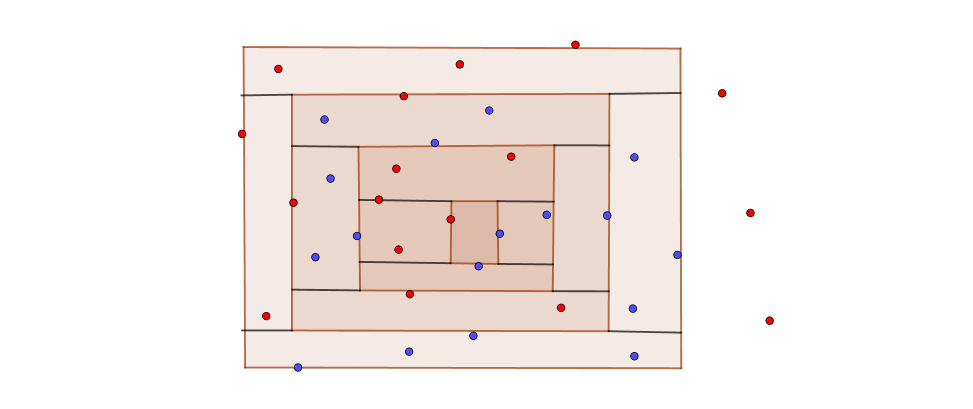
\includegraphics[width=\textwidth]{Construccion-poligono-2-alternancia-3}
\end{figure}
\end{frame}
\begin{frame}
\begin{figure}[h]
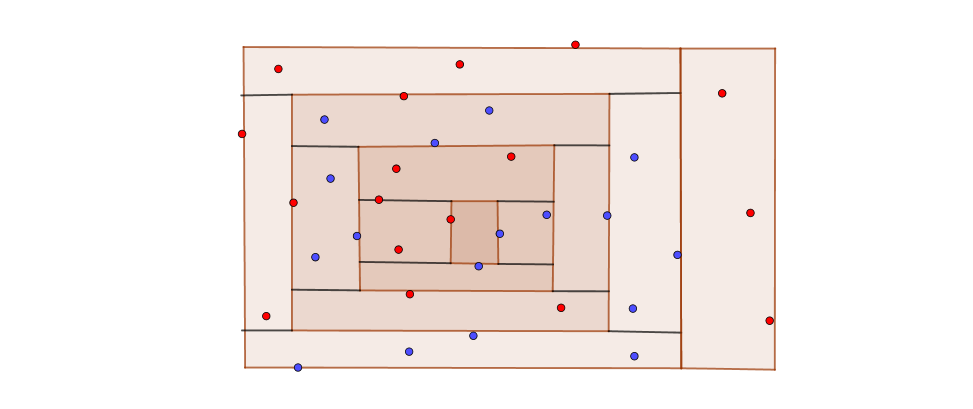
\includegraphics[width=\textwidth]{Construccion-poligono-2-alternancia-4}
\end{figure}
\end{frame}
\begin{frame}
\begin{figure}[h]
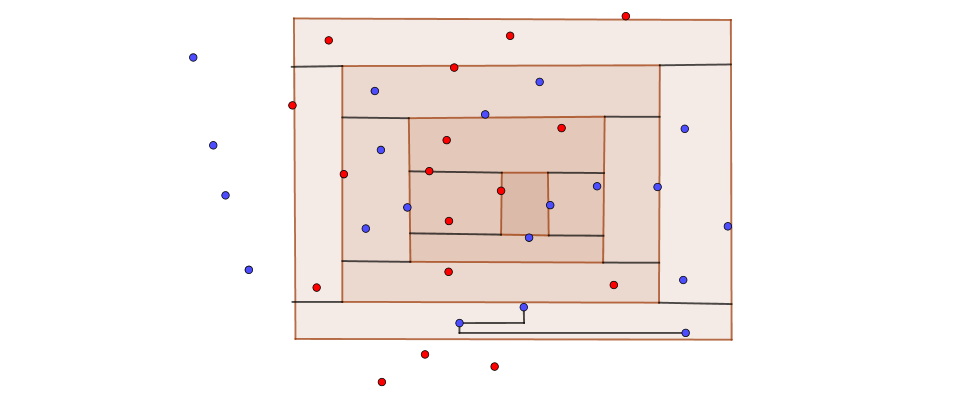
\includegraphics[width=\textwidth]{Construccion-poligono-2-alternancia-deco}
\end{figure}
\end{frame}
\begin{frame}
\begin{figure}[h]
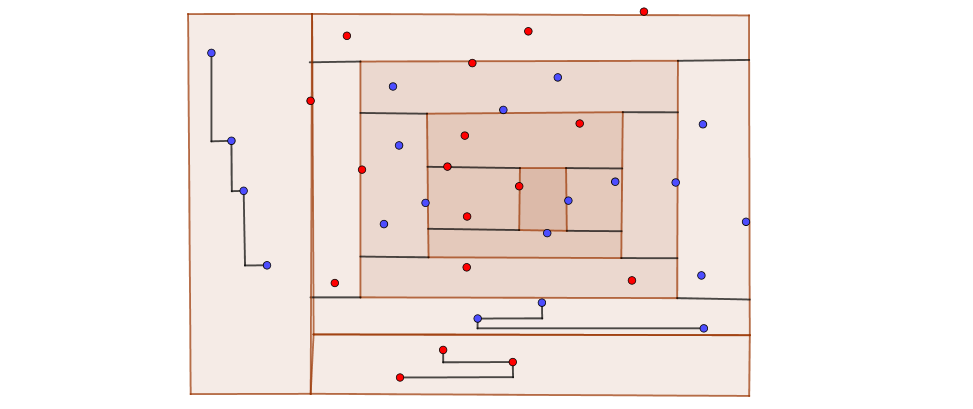
\includegraphics[width=\textwidth]{Construccion-poligono-2-alternancia-deco-2}
\end{figure}
\end{frame}
\begin{frame}
\begin{figure}[h]
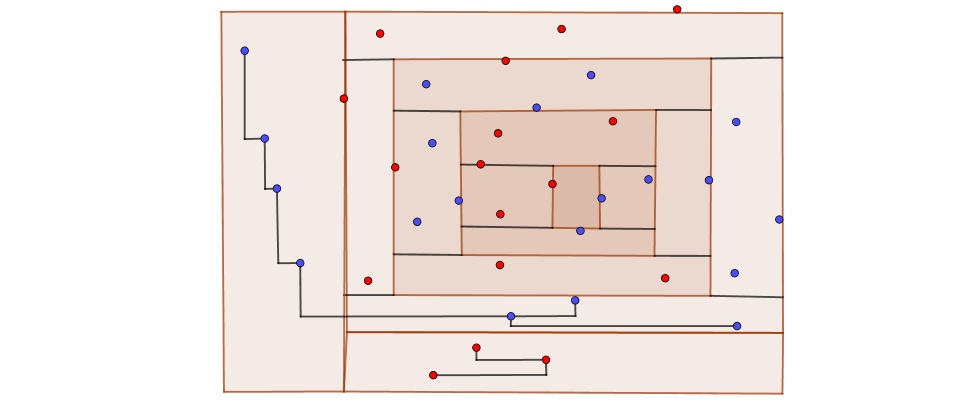
\includegraphics[width=\textwidth]{Construccion-poligono-2-alternancia-deco-3}
\end{figure}
\end{frame}
\begin{frame}
\begin{figure}[h]
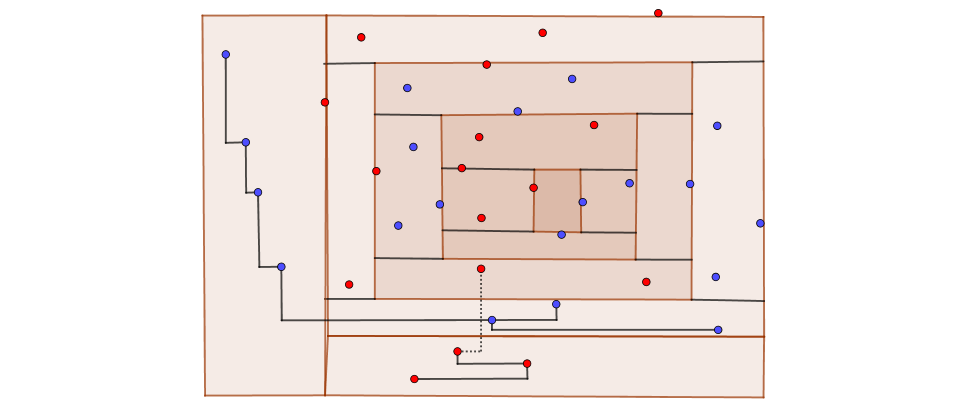
\includegraphics[width=\textwidth]{Construccion-poligono-2-alternancia-deco-4}
\end{figure}
\end{frame}
\begin{frame}
\begin{figure}[h]
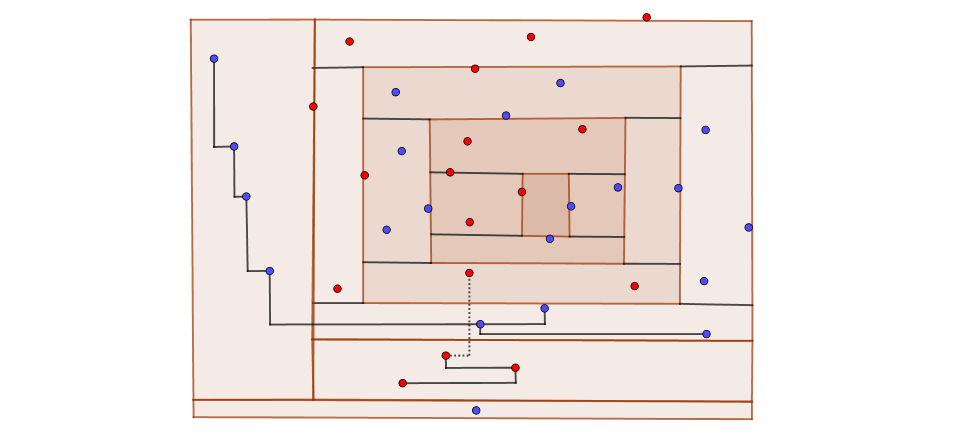
\includegraphics[width=\textwidth]{Construccion-poligono-2-alternancia-deco-5}
\end{figure}
\end{frame}
\begin{frame}
\begin{figure}[h]
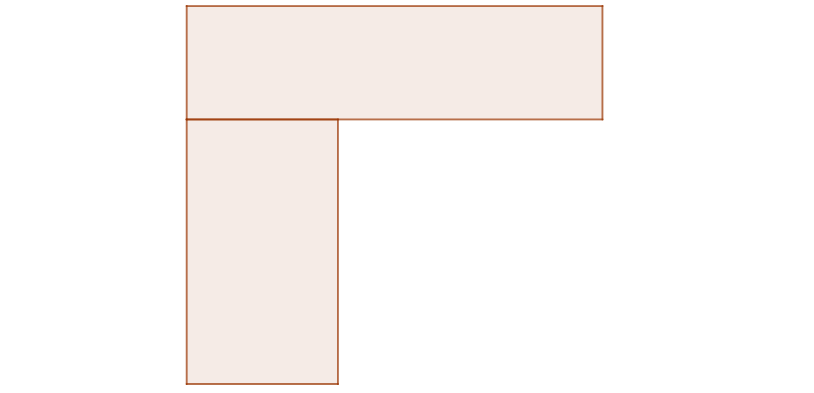
\includegraphics[width=\textwidth]{Nuestra-construccion}
\end{figure}
\end{frame}
\begin{frame}
\begin{figure}[h]
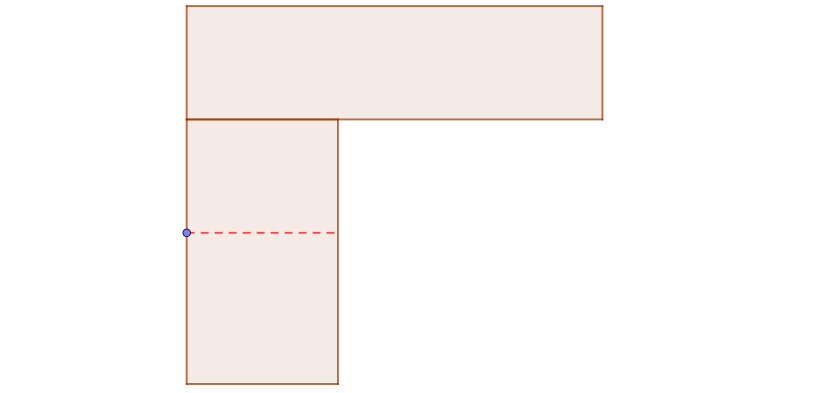
\includegraphics[width=\textwidth]{Nuestra-construccion-2}
\end{figure}
\end{frame}
\begin{frame}
\begin{figure}[h]
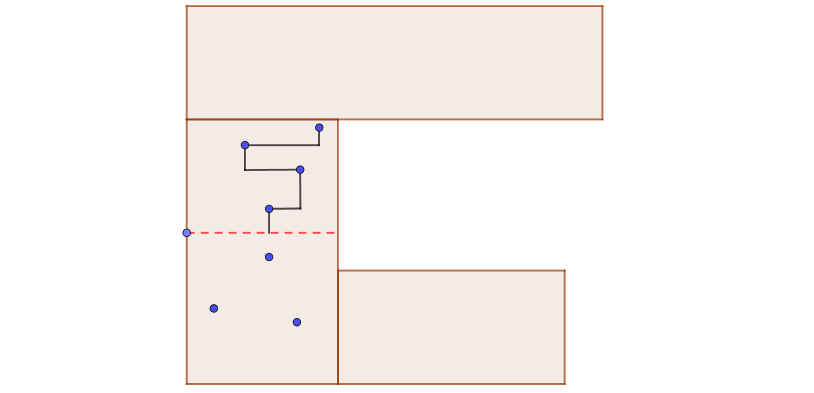
\includegraphics[width=\textwidth]{Nuestra-construccion-3}
\end{figure}
\end{frame}
\begin{frame}
\begin{figure}[h]
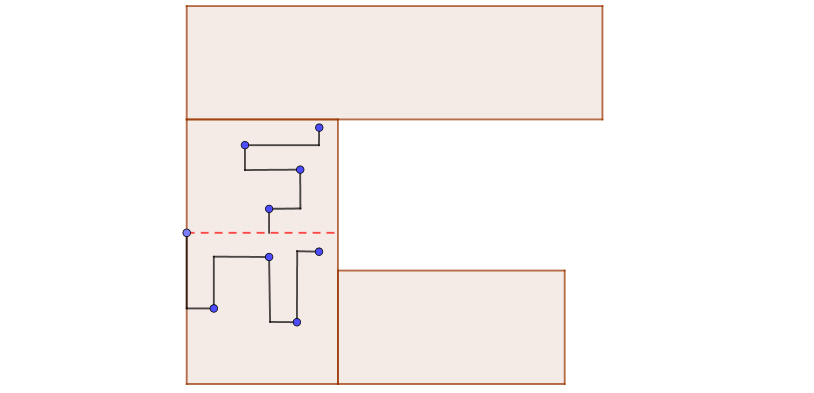
\includegraphics[width=\textwidth]{Nuestra-construccion-4}
\end{figure}
\end{frame}
\begin{frame}
\begin{figure}[h]
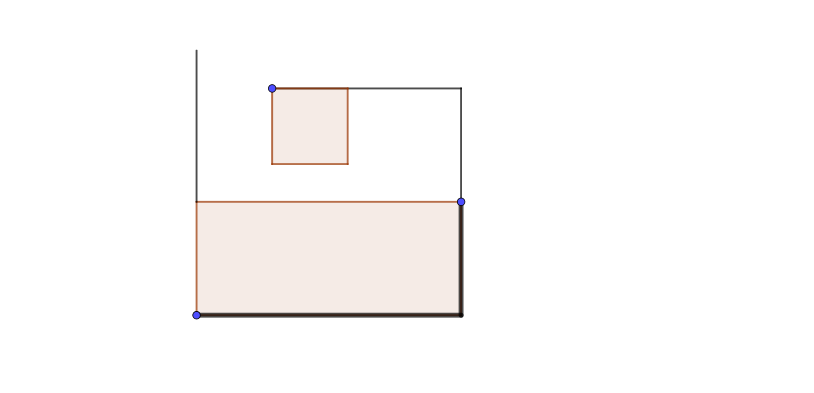
\includegraphics[width=\textwidth]{Cajas-2-puntos}
\end{figure}
\end{frame}
\begin{frame}
\begin{figure}[h]
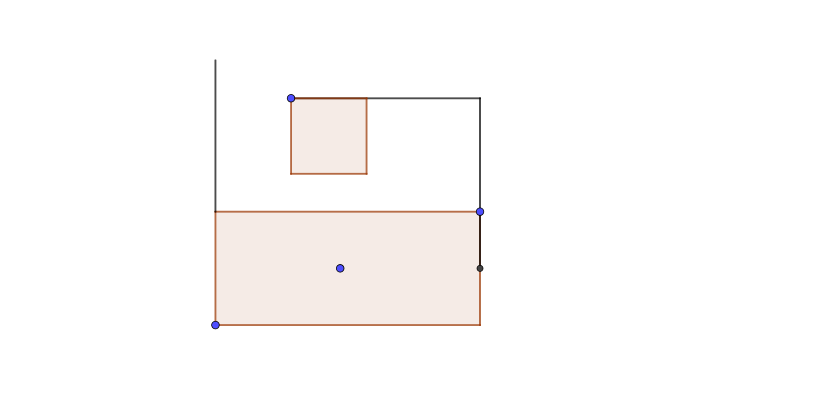
\includegraphics[width=\textwidth]{Cajas-3-puntos-si-puede}
\end{figure}
\end{frame}
\begin{frame}
\begin{figure}[h]
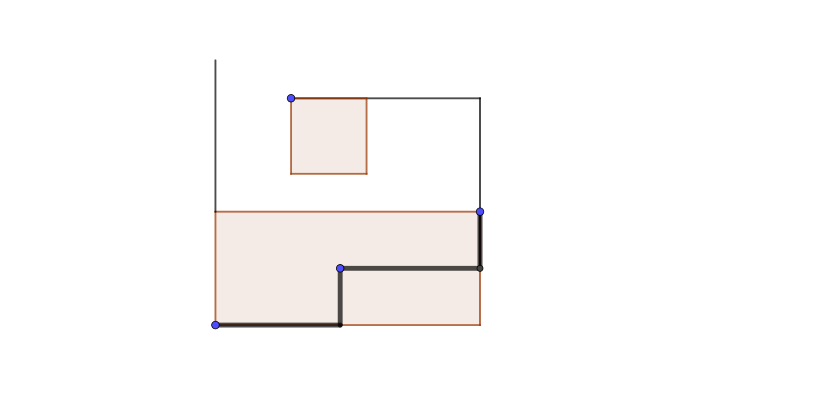
\includegraphics[width=\textwidth]{Cajas-3-puntos-si-puede-2}
\end{figure}
\end{frame}
\begin{frame}
\begin{figure}[h]
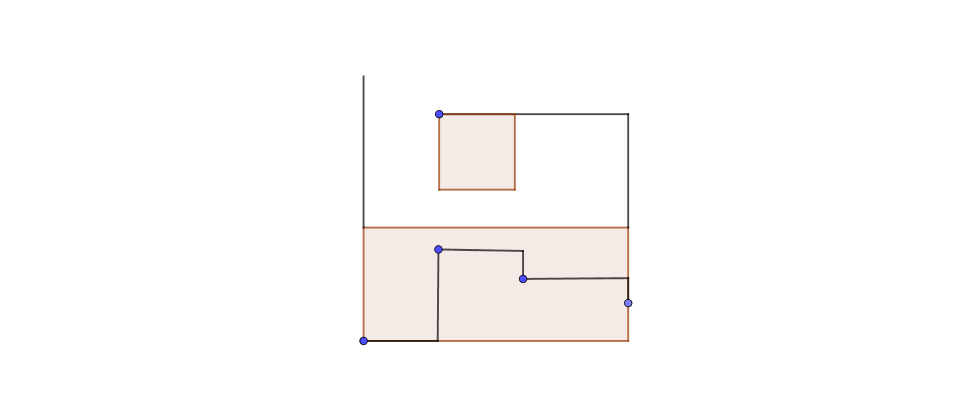
\includegraphics[width=\textwidth]{Cajas-4-puntos}
\end{figure}
\end{frame}
\begin{frame}
\begin{figure}[h]
\includegraphics[width=\textwidth]{Cajas-4-puntos-2}
\end{figure}
\end{frame}
\begin{frame}
\begin{figure}[h]
\includegraphics[width=\textwidth]{Cajas-4-puntos-3}
\end{figure}
\end{frame}
\begin{frame}
\begin{figure}[h]
\includegraphics[width=\textwidth]{Cajas-3-puntos-no-puede}
\end{figure}
\end{frame}
\begin{frame}
\begin{figure}[h]
\includegraphics[width=\textwidth]{Cajas-3-puntos-no-puede-2}
\end{figure}
\end{frame}
\begin{frame}
\begin{figure}[h]
\includegraphics[width=\textwidth]{Cajas-3-puntos-no-puede-3}
\end{figure}
\end{frame}
\begin{frame}
\begin{figure}[h]
\includegraphics[width=\textwidth]{Caso-de-n-cuartos-steiner}
\end{figure}
\end{frame}
\begin{frame}
\begin{figure}[h]
\includegraphics[width=\textwidth]{Caso-de-n-cuartos-steiner-2}
\end{figure}
\end{frame}
\begin{frame}
\begin{figure}[h]
\includegraphics[width=\textwidth]{Caso-de-n-cuartos-steiner-3}
\end{figure}
\end{frame}
\begin{frame}
\begin{figure}[h]
\includegraphics[width=\textwidth]{Caso-de-n-cuartos-steiner-4}
\end{figure}
\end{frame}
\begin{frame}
\begin{figure}[h]
\includegraphics[width=\textwidth]{Caso-de-n-cuartos-steiner-5}
\end{figure}
\end{frame}
\begin{frame}
\begin{figure}[h]
\includegraphics[width=6cm, height=6cm]{ejemplo-trayectoria}
\end{figure}
\end{frame}
%\begin{frame}
%\printbibliography
%\end{frame}
\begin{frame}
\begin{center}
\begin{Huge}
Gracias!
\end{Huge}
\end{center}
\end{frame}




\end{document}